\documentclass[12pt,a4paper,oneside]{report}             % Single-side
%\documentclass[11pt,a4paper,twoside,openright]{report}  % Duplex

%\PassOptionsToPackage{chapternumber=Huordinal}{magyar.ldf} %betuvel a fejezetek szama
\usepackage{t1enc}
%\usepackage[latin2]{inputenc}
\usepackage{amsmath}
\usepackage{amssymb}
\usepackage{enumerate}
\usepackage[thmmarks]{ntheorem}
\usepackage{graphics}
\usepackage{epsfig}
\usepackage{listings}
\usepackage{color}
%\usepackage{fancyhdr}
\usepackage{lastpage}
\usepackage{anysize}
\usepackage[magyar]{babel}
\usepackage[utf8]{inputenc}
\usepackage{sectsty}
\usepackage{setspace}  % Ettol a tablazatok, abrak, labjegyzetek maradnak 1-es sorkozzel!
\usepackage[hang]{caption}
\usepackage{hyperref}
\usepackage{float} % ezzel lehet helybe rakni az abrat
\usepackage{listings}

\usepackage{subfig}

\usepackage{array}
\usepackage{multirow}
\usepackage{mdwlist}
\makecompactlist{myitemize*}{itemize}

%--------------------------------------------------------------------------------------
% Main variables
%--------------------------------------------------------------------------------------
\newcommand{\vikszerzo}{Bakró Nagy István}
\newcommand{\vikkonzulens}{Hartmann Péter \& Reichardt András}
\newcommand{\vikcim}{Poros plazma kísérletek támogatása multiprocesszoros környezetben}
\newcommand{\viktanszek}{Szélessávú Hírközlés és Villamosságtan Tanszék}
\newcommand{\vikdoktipus}{Diplomatervezés 1. - beszámoló}
\newcommand{\vikdepartmentr}{Szélessávú Hírközlés és Villamosságtan Tanszék}

%--------------------------------------------------------------------------------------
% Page layout setup
%--------------------------------------------------------------------------------------
% we need to redefine the pagestyle plain
% another possibility is to use the body of this command without \fancypagestyle
% and use \pagestyle{fancy} but in that case the special pages
% (like the ToC, the References, and the Chapter pages)remain in plane style

\pagestyle{plain}
%\setlength{\parindent}{0pt} % áttekinthet?bb, angol nyelv? dokumentumokban
% jellemz? \setlength{\parskip}{8pt plus 3pt minus 3pt} % áttekinthet?bb, angol nyelv? dokumentumokban jellemz?
\setlength{\parindent}{30pt} % magyar nyelv? dokumentumokban jellemz?
\setlength{\parskip}{0pt}    % magyar nyelv? dokumentumokban jellemz?

\marginsize{35mm}{25mm}{15mm}{15mm} % anysize package
\setcounter{secnumdepth}{0}
\sectionfont{\large\upshape\bfseries}
\setcounter{secnumdepth}{2}
\singlespacing
\frenchspacing

%--------------------------------------------------------------------------------------
%	Setup hyperref package
%--------------------------------------------------------------------------------------
\hypersetup{
    bookmarks=true,            % show bookmarks bar?
    unicode=false,             % non-Latin characters in Acrobat’s bookmarks
    pdftitle={\vikcim},        % title
    pdfauthor={\vikszerzo},    % author
    pdfsubject={\vikdoktipus}, % subject of the document
    pdfcreator={\vikszerzo},   % creator of the document
    pdfproducer={Producer},    % producer of the document
    pdfkeywords={keywords},    % list of keywords
    pdfnewwindow=true,         % links in new window
    %pdfborder={1 2 3},
    colorlinks=true,           % false: boxed links; true: colored links
    linkcolor=black,           % color of internal links
    citecolor=black,           % color of links to bibliography
    filecolor=black,           % color of file links
    urlcolor=black             % color of external links
}

%--------------------------------------------------------------------------------------
% Set up listings
%--------------------------------------------------------------------------------------
\lstset{
	basicstyle=\scriptsize\ttfamily, % print whole listing small
	keywordstyle=\color{black}\bfseries\underbar, % underlined bold black keywords
	identifierstyle=, 					% nothing happens
	commentstyle=\color{white}, % white comments
	stringstyle=\scriptsize\sffamily, 			% typewriter type for strings
	showstringspaces=false,     % no special string spaces
	aboveskip=3pt,
	belowskip=3pt,
	columns=fixed,
	backgroundcolor=\color{lightgray},
} 		
\def\lstlistingname{lista}	

%--------------------------------------------------------------------------------------
%	Some new commands and declarations
%--------------------------------------------------------------------------------------
\newcommand{\code}[1]{{\upshape\ttfamily\scriptsize\indent #1}}

% define references
\newcommand{\figref}[1]{\ref{fig:#1}.}
\renewcommand{\eqref}[1]{(\ref{eq:#1})}
\newcommand{\listref}[1]{\ref{listing:#1}.}
\newcommand{\sectref}[1]{\ref{sect:#1}}
\newcommand{\tabref}[1]{\ref{tab:#1}.}


\newcommand{\ud}{\ \mathrm{d}}
\newcommand{\mhat}[1]{\mathrm{\hat{#1}}}
\renewcommand{\vec}[1]{\overrightarrow{\mathrm{#1}}}

\DeclareMathOperator*{\argmax}{arg\,max}
%\DeclareMathOperator*[1]{\floor}{arg\,max}
\DeclareMathOperator{\sign}{sgn}
\DeclareMathOperator{\rot}{rot}
\definecolor{lightgray}{rgb}{0.95,0.95,0.95}

\author{\vikszerzo}
\title{\viktitle}
%--------------------------------------------------------------------------------------
%	Setup captions
%--------------------------------------------------------------------------------------
\captionsetup[figure]{
%labelsep=none,
%font={footnotesize,it},
%justification=justified,
width=.75\textwidth,
aboveskip=10pt}

\renewcommand{\captionlabelfont}{\small\bf}
\renewcommand{\captionfont}{\footnotesize\it}

%--------------------------------------------------------------------------------------
% Table of contents and the main text
%--------------------------------------------------------------------------------------
\begin{document}
\singlespacing
%\include{guideline}


%\pagenumbering{arabic}
%\pagenumbering{roman}
\onehalfspacing
\setcounter{page}{999}
%--------------------------------------------------------------------------------------
%	The title page
%--------------------------------------------------------------------------------------
\begin{titlepage}
\begin{center}
%
\includegraphics[width=60mm,keepaspectratio]{figures/BMElogo.png}\\
\vspace{0.3cm}
\textbf{Budapesti Mûszaki és Gazdaságtudományi Egyetem}\\
\textmd{Villamosmérnöki és Informatikai Kar}\\
\textmd{\viktanszek}\\[5cm]

\vspace{0.4cm}
{\huge \bfseries \vikcim}\\[0.8cm]
\vspace{0.5cm}
\textsc{\Large \vikdoktipus}\\[4cm]

\begin{tabular}{cc}
 \makebox[7cm]{\emph{Készítette}} & \makebox[7cm]{\emph{Konzulens}} \\
 \makebox[7cm]{\vikszerzo} & \makebox[7cm]{\vikkonzulens}
\end{tabular}

\vfill
{\large \today}
\end{center}
\end{titlepage}
\clearpage

\pagenumbering{roman}
\setcounter{page}{1}
\pdfbookmark{\contentsname}{toc}
\tableofcontents%\addcontentsline{toc}{chapter}{Tartalomjegyzék}
\clearpage
%\include{declaration}

%--------------------------------------------------------------------------------------
% Feladatkiiras (a tanszeken atveheto, kinyomtatott valtozat)
%--------------------------------------------------------------------------------------
\clearpage
\begin{center}
\large
\textbf{FELADATKIÍRÁS}\\
\end{center}

\noindent A GPU kártyák teljesítményének növekedése magas potenciált jelent a 
szimulátorok készítésében.
Ezzel egyetemben más programozási metodika is kívánkozik hozzá.\\

\noindent A hallgató feladatának a következõkre kell kiterjednie:
\begin{itemize}
\item Válasszon egy problémát szimulálásra és mutassa be a modelljét
\item Mutassa be a CUDA számítási platformját és a programozási metodikáját
\item Készítsen szimulációs programot MATLAB és CUDA platformon
\item Vizsgálja meg a kettő számítási teljesítményét és számítási pontosságát
\item Adjon iránymutatást a szimulátor további fejlesztési irányához!
\end{itemize}

\begin{flushleft}
\vspace*{1cm}
\textbf{Tanszéki konzulens}: Reichardt András, egy. tanársegéd
\end{flushleft}

\begin{flushleft}
\vspace*{1cm}
Budapest, 2013. szeptember 9.
\end{flushleft}

\clearpage

\pagenumbering{arabic}
\setcounter{page}{1}

% %----------------------------------------------------------------------------
% Abstract in hungarian
%----------------------------------------------------------------------------
\chapter*{Kivonat}\addcontentsline{toc}{chapter}{Kivonat}

hablaty

\vfill

% \include{introduction}
%----------------------------------------------------------------------------
\chapter{A poros plazma kísérlet}
%----------------------------------------------------------------------------
\section{Bevezető}
	A poros plazma kísérlet ionizált nemesgáz és az abba szórt porrészecskék megfigyeléséből áll.
	Adott alacsony nyomású gáz terében elhelyezett elektródákra kapcsolt váltakozó feszültséggel 
	lehetséges plazmát létrehozni. A váltakozó villamos tér a töltéssel rendelkező elektronokra 
	olyan erővel hat, hogy azok leszakadnak az atomról ezzel ionizálva azokat.
	A leszakadó elektronok a térben szabadon a ráható erőknek megfelelően mozognak.
	Ez makroszkópikus skálán a gáz vezetővé válását jelenti. A szabad elektronok mozgásának
	során az ionizált atomokon szórodnak, ami ködfénykisüléshez vezet. 
	
	A kísérlet során az előbb ismertett plazma terébe porrészecskéket szórunk. A porrészecskék alatt
	$10nm - 100\mu m$ nagyságú részecskéket értünk, például $SiO_2$, $Al_2O_3$ vagy 
	melamine-formaldehyde-t. A porrészecskék a plazmával interakcióba lépve negatívan feltöltődnek.
	A porrészecskék töltésének és tömegének hányadosa a szabad elektronokhoz és az ionokhoz képest
	sokkal kissebb, ezáltal a mozgására való hatása elhanyagolható.
	
	A porrészecskék transzportjának megértéséhez szükséges a ráható erők azonosítása.
	A különféle erők nagysága a porrészecskék nagyságától különféleképpen skálázódik. Elhanyagolásokat
	ennek megfelelően tehetünk.
	\begin{description}
		\item[Gravitációs $F_g$ erő:] Mikrogravitációban végzett kísérletek kivételével a porrészecskére
			ható gravitációs erő lineárisan arányos a tömegével. Nanométer nagyságú részecskék esetén
			elhanyagolható, de a jelen esetben használt mikrométer nagyságú részecskék esetén dominánsak,
		\item[Villamos tér keltette $F_e$ erő:] A porrészecske töltésével és a villamos tér nagyságával
			arányos. A megfelelően irányított villamos térrel lehetséges a részecskék levitációja,  
		\item[Háttératomon való szóródás $F_n$:] A porrészecske driftje során a háttératomokkal való
			szóródásának makroszkópikus erőként való számításba vétele,
		\item[Hőmérséklet gradiensi $F_{th}$ erő:] A gáz hőmérsékletének gradiense okozta
			gázatomok diffúzív jellegű mozgása által okozott indirekt erőhatás,
		\item[Ion sodrási $F_i$ erő:] Az ionokra ható villamos tér okozta erőnek indirekt hatása a
			porrészecskékre.
	\end{description}
	A poros plazma analízise során fontos szerepet játszik a porrészecskék csatolása.
	A csatolást gyengének és erősnek kategorizáljuk aszerint, hogy a részecskék szomszédja általi
	átlagos potenciális energia az átlagos termikus (kinetikus) energiájához képest kissebb vagy
	nagyobb.
	A csatolást a Coulomb csatolási paraméterrel ($\Gamma$) lehet számosítani, ami a szomszédos
	részecskék Coulomb potenciáljának és termikus energiájának hatványa:
	\begin{equation}
		\Gamma = \cfrac{Q^2 / 4\pi\varepsilon_0 d}{kT_d} 
	\end{equation}
	ahol $Q$ a részecskék töltése, $d$ az átlagos részecske távolság és a $T_d$ a por hőmérséklete.
	Ha a $\Gamma$ értéke egy kritikus érték fölé $\Gamma > 150$ növekszik, akkor
	Ikawa jóslata szerint a porrészecskék Coulomb kristályszerkezetbe rendeződik.
	
	Az iparban anyag porlasztására és mintázat maratására használják. Továbbá szennyeződésként a VLSI
	áramkörök gyártásakor jelentkezik, ami a kihozatal csökkenését és a teljesítmény csökkenéséhez
	vezet. Laboratóriumi környezetben kristály halmazállapot változását, viszkozitását lehet kutatni. 

%----------------------------------------------------------------------------
\section{A kísérlet}
%----------------------------------------------------------------------------
	A kísérlet lebonyolítására egy speciális kamrára van szükség, amiben lehetséges a plazma
	létrehozása, a porrészecskék szórása illetve a megfelelő villamos tér létrehozása.
	A kamrának hermetikusan jól zártnak kell lennie, hogy csak a kívánt gázt tartalmazza.
	A középvákuumú működéshez kétlépéses vákuumszivattyút kell alkalmazni.
	
	
	
	A kamra sematikus ábrája a \ref{fig:meresch}. ábrán látható.
	A porrészecskék levitációjáért a villamos tér felelős. A síkba való zárás parabolikus
	potenciállal lehetséges. Az ilyen tér létrehozása a következő elektróda elrendezéssel lehetséges:
	alul elhelyezett korong alakú elektróda, ami felett egy gyűrű alakú elektróda helyezkedik el.
	Az ilyen elektródarendszerre kapcsolt váltakozó feszültség a beszórt porrészecskéket lebegtetni
	tudja. Továbbá a részecskék követéséhez lézerrel megvilágítjuk és nagysebességű kamerával
	felvételt készítünk róla.
	
	\begin{figure}[H]
		\centering
		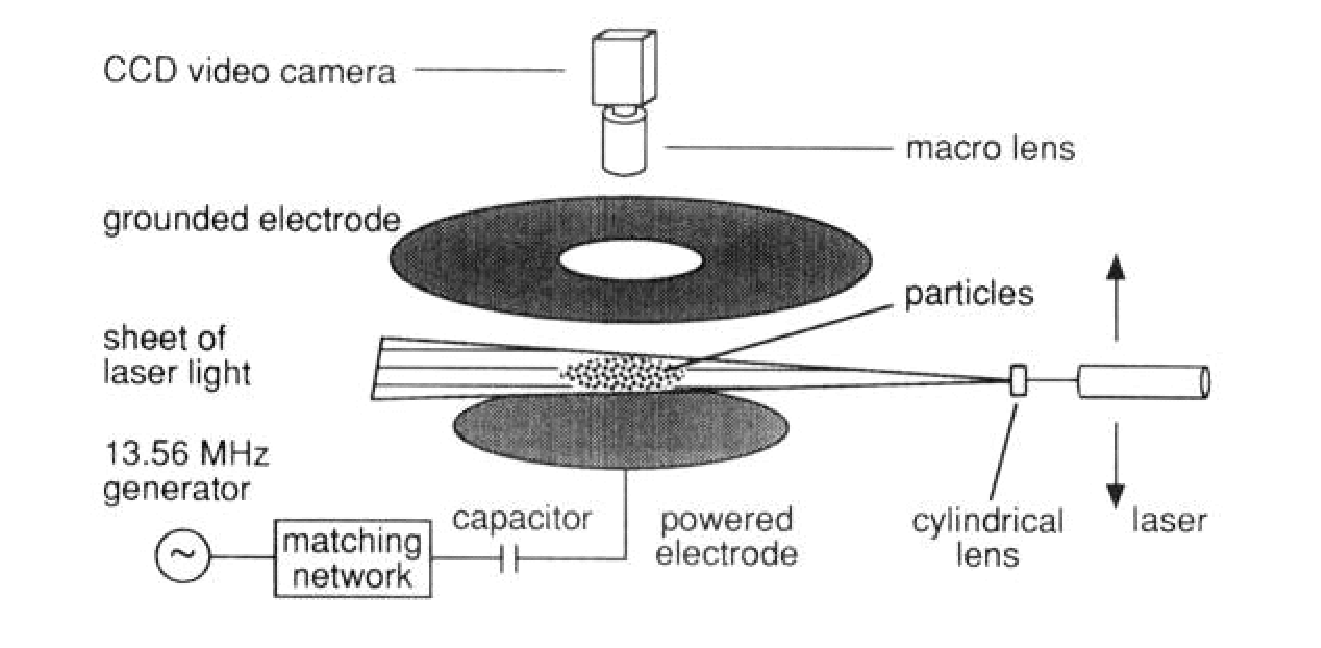
\includegraphics[width=0.9\columnwidth]{figures/eps/dust_camera.eps}
		\caption{A mérési elrendezés sematikus ábrája (forrás: \cite{Merlino2006})} 
		\label{fig:meresch}
	\end{figure}
	
	A kamrát (\ref{fig:kamra}. ábra) Hartmann Péter külső konzulensem építette és a MTA Wigner FK SZFI
	Gázkisülési Laboratóriumában található.
	
	\noindent A paraméterei:
	\begin{myitemize*}
		\item Kamra belső átmérője: $25cm$
		\item Kamra belső magassága: $18cm$
		\item Alsó elektróda átmérője: $18cm$
		\item Felső gyűrű elektróda belső átmérője: $15cm$
		\item Felső elektróda távolsága az alsótól: $13cm$
		\item Argon gáz nyomása: $1.2\pm0.05 Pa$
		\item Gáz átfolyása: $\sim 0.01 CCPM$
		\item RF gerjesztés: $7W\ @ \ 13.56 MHz$
		\item Porrészecske: melamine-formaldehyde
		\item Porrészecske átmérője: $4.38\pm 0.06 \mu m$
		\item Porrészecske tömege. $6.64\cdot10^{-14} kg$
		\item Látható porrészecskék száma: $\sim 2500$
		\item Megvilágító lézer: $200mW\quad @ \quad 532nm$
		\item Kamera: $1.4MPixel\ @\ 100 FPS$
	\end{myitemize*}
	A kamra alsó elektródáját lehetséges egy motorral forgásba hozni. Ezáltal a kamrában lévő gáz is
	forgásba jön, ami a porrészecskékre az $F_i$ ionsodrási erővel hatva nagy mágneses tér Lorentz
	erejének feleltethető meg.
	\begin{figure}[H]
		\centering
		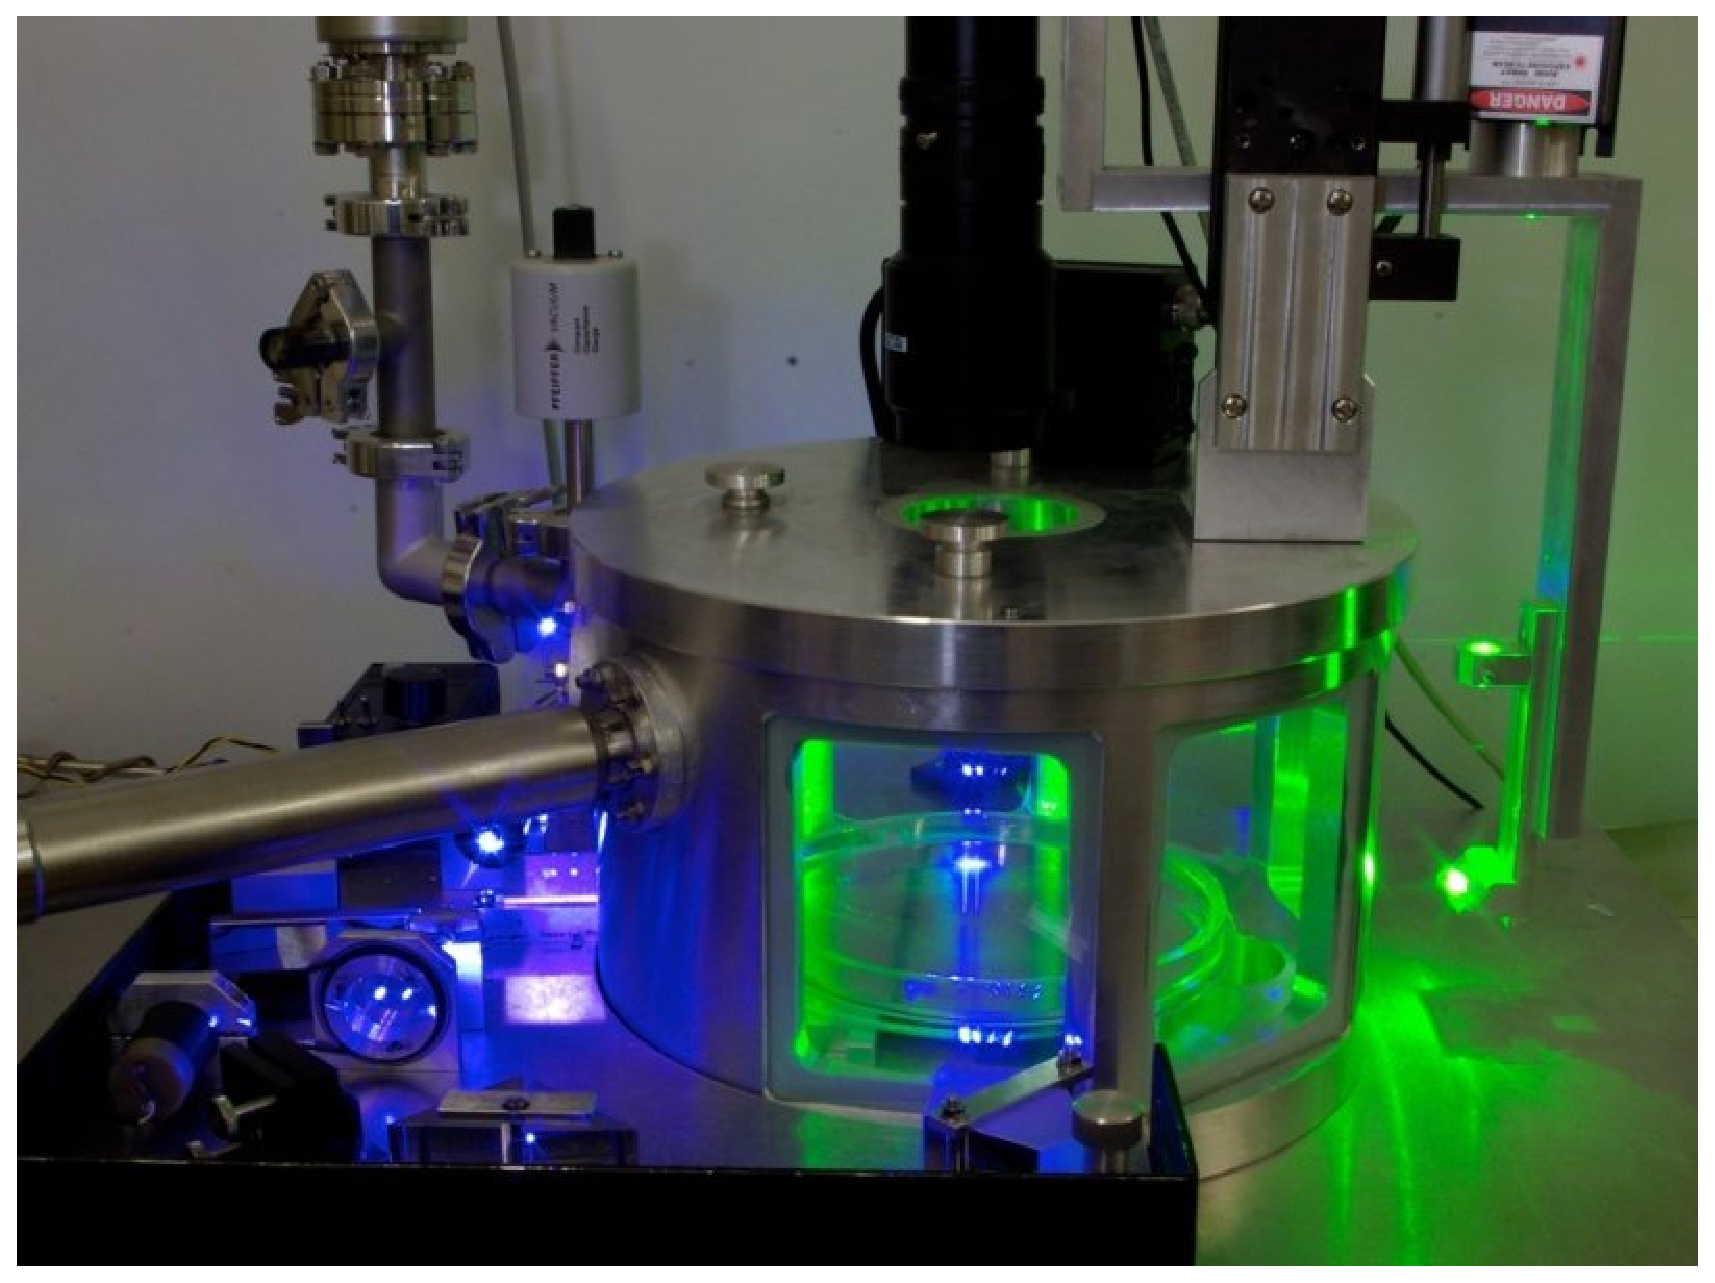
\includegraphics[width=0.9\columnwidth]{figures/eps/dusty2.eps}
		\caption{A konkrét kamra működése közben} 
		\label{fig:kamra}
	\end{figure}
	
%----------------------------------------------------------------------------
\section{A mérendő mennyiségek és a származtatott értékek}
%----------------------------------------------------------------------------
	A kísérlet előkészítése a következő lépésekből áll:
	\begin{enumerate*}
		\item Elővákum szivattyú bekapcsolása,
		\item Középvákuum szivattyú bekapcsolása,
		\item Argon palack megnyitása a megfelelő áramlás szintjére,
		\item RF gerjesztés bekapcsolása,
		\item Megvilágító lézer bekapcsolása,
		\item \label{it:por} Porrészecskék beszórása,
		\item Kamera bekapcsolása és a megjelenítő szoftver futtatása,
		\item Ha sok összetapadt porrészecske látható, illetve ha túl sok porrészecske látható, akkor
		az RF gerjesztés gyors ki-be kapcsolása után a \ref{it:por}.-től való folytatása a folyamatnak.
	\end{enumerate*}
	A \ref{fig:captures}. ábrán látható álló és forgó alsó elektródájú kísérlet során a
	porrészecskékről készült kép.
	
	\begin{figure}[H]
		\centering
		\subfloat[Álló elektróda esetén sok $\left(\sim 1500\right)$ részecske]{
			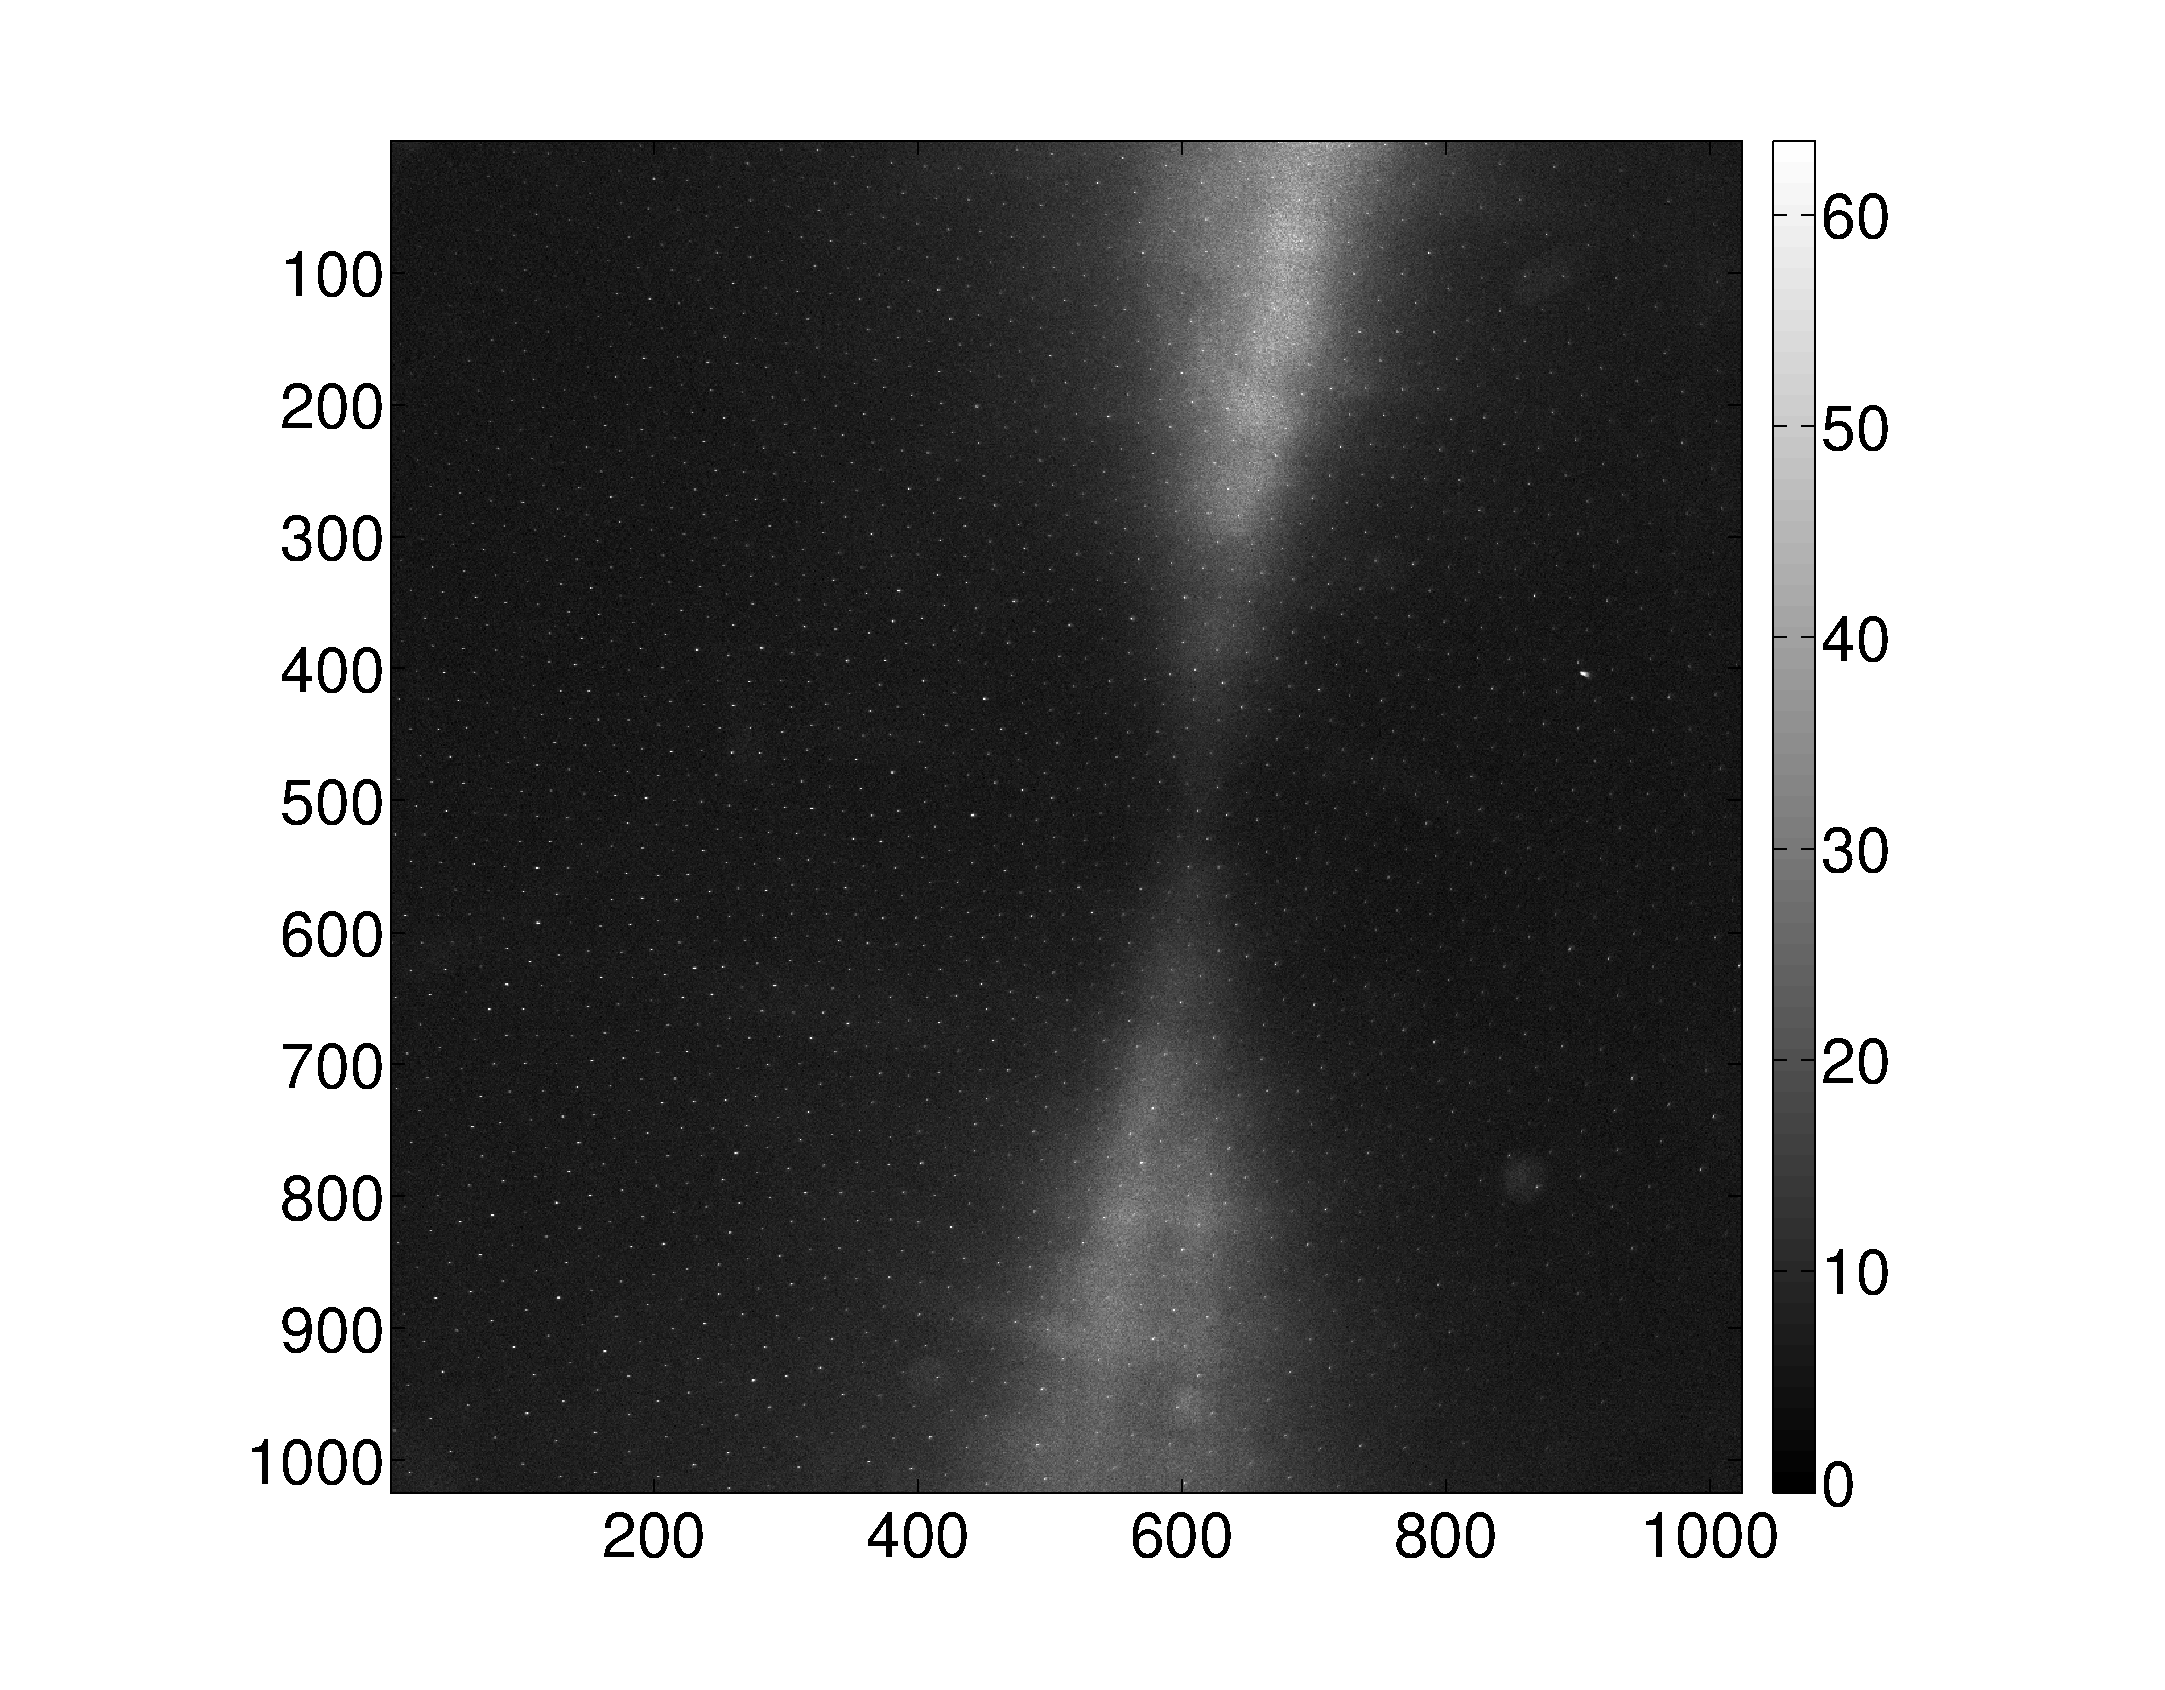
\includegraphics[width=0.95\columnwidth]{figures/eps/000047659380.eps}%
			\label{fig:allo}
		}
		\\
		\subfloat[Forgó elektróda esetén kevés $\left(\sim 100\right)$ részecske]{
			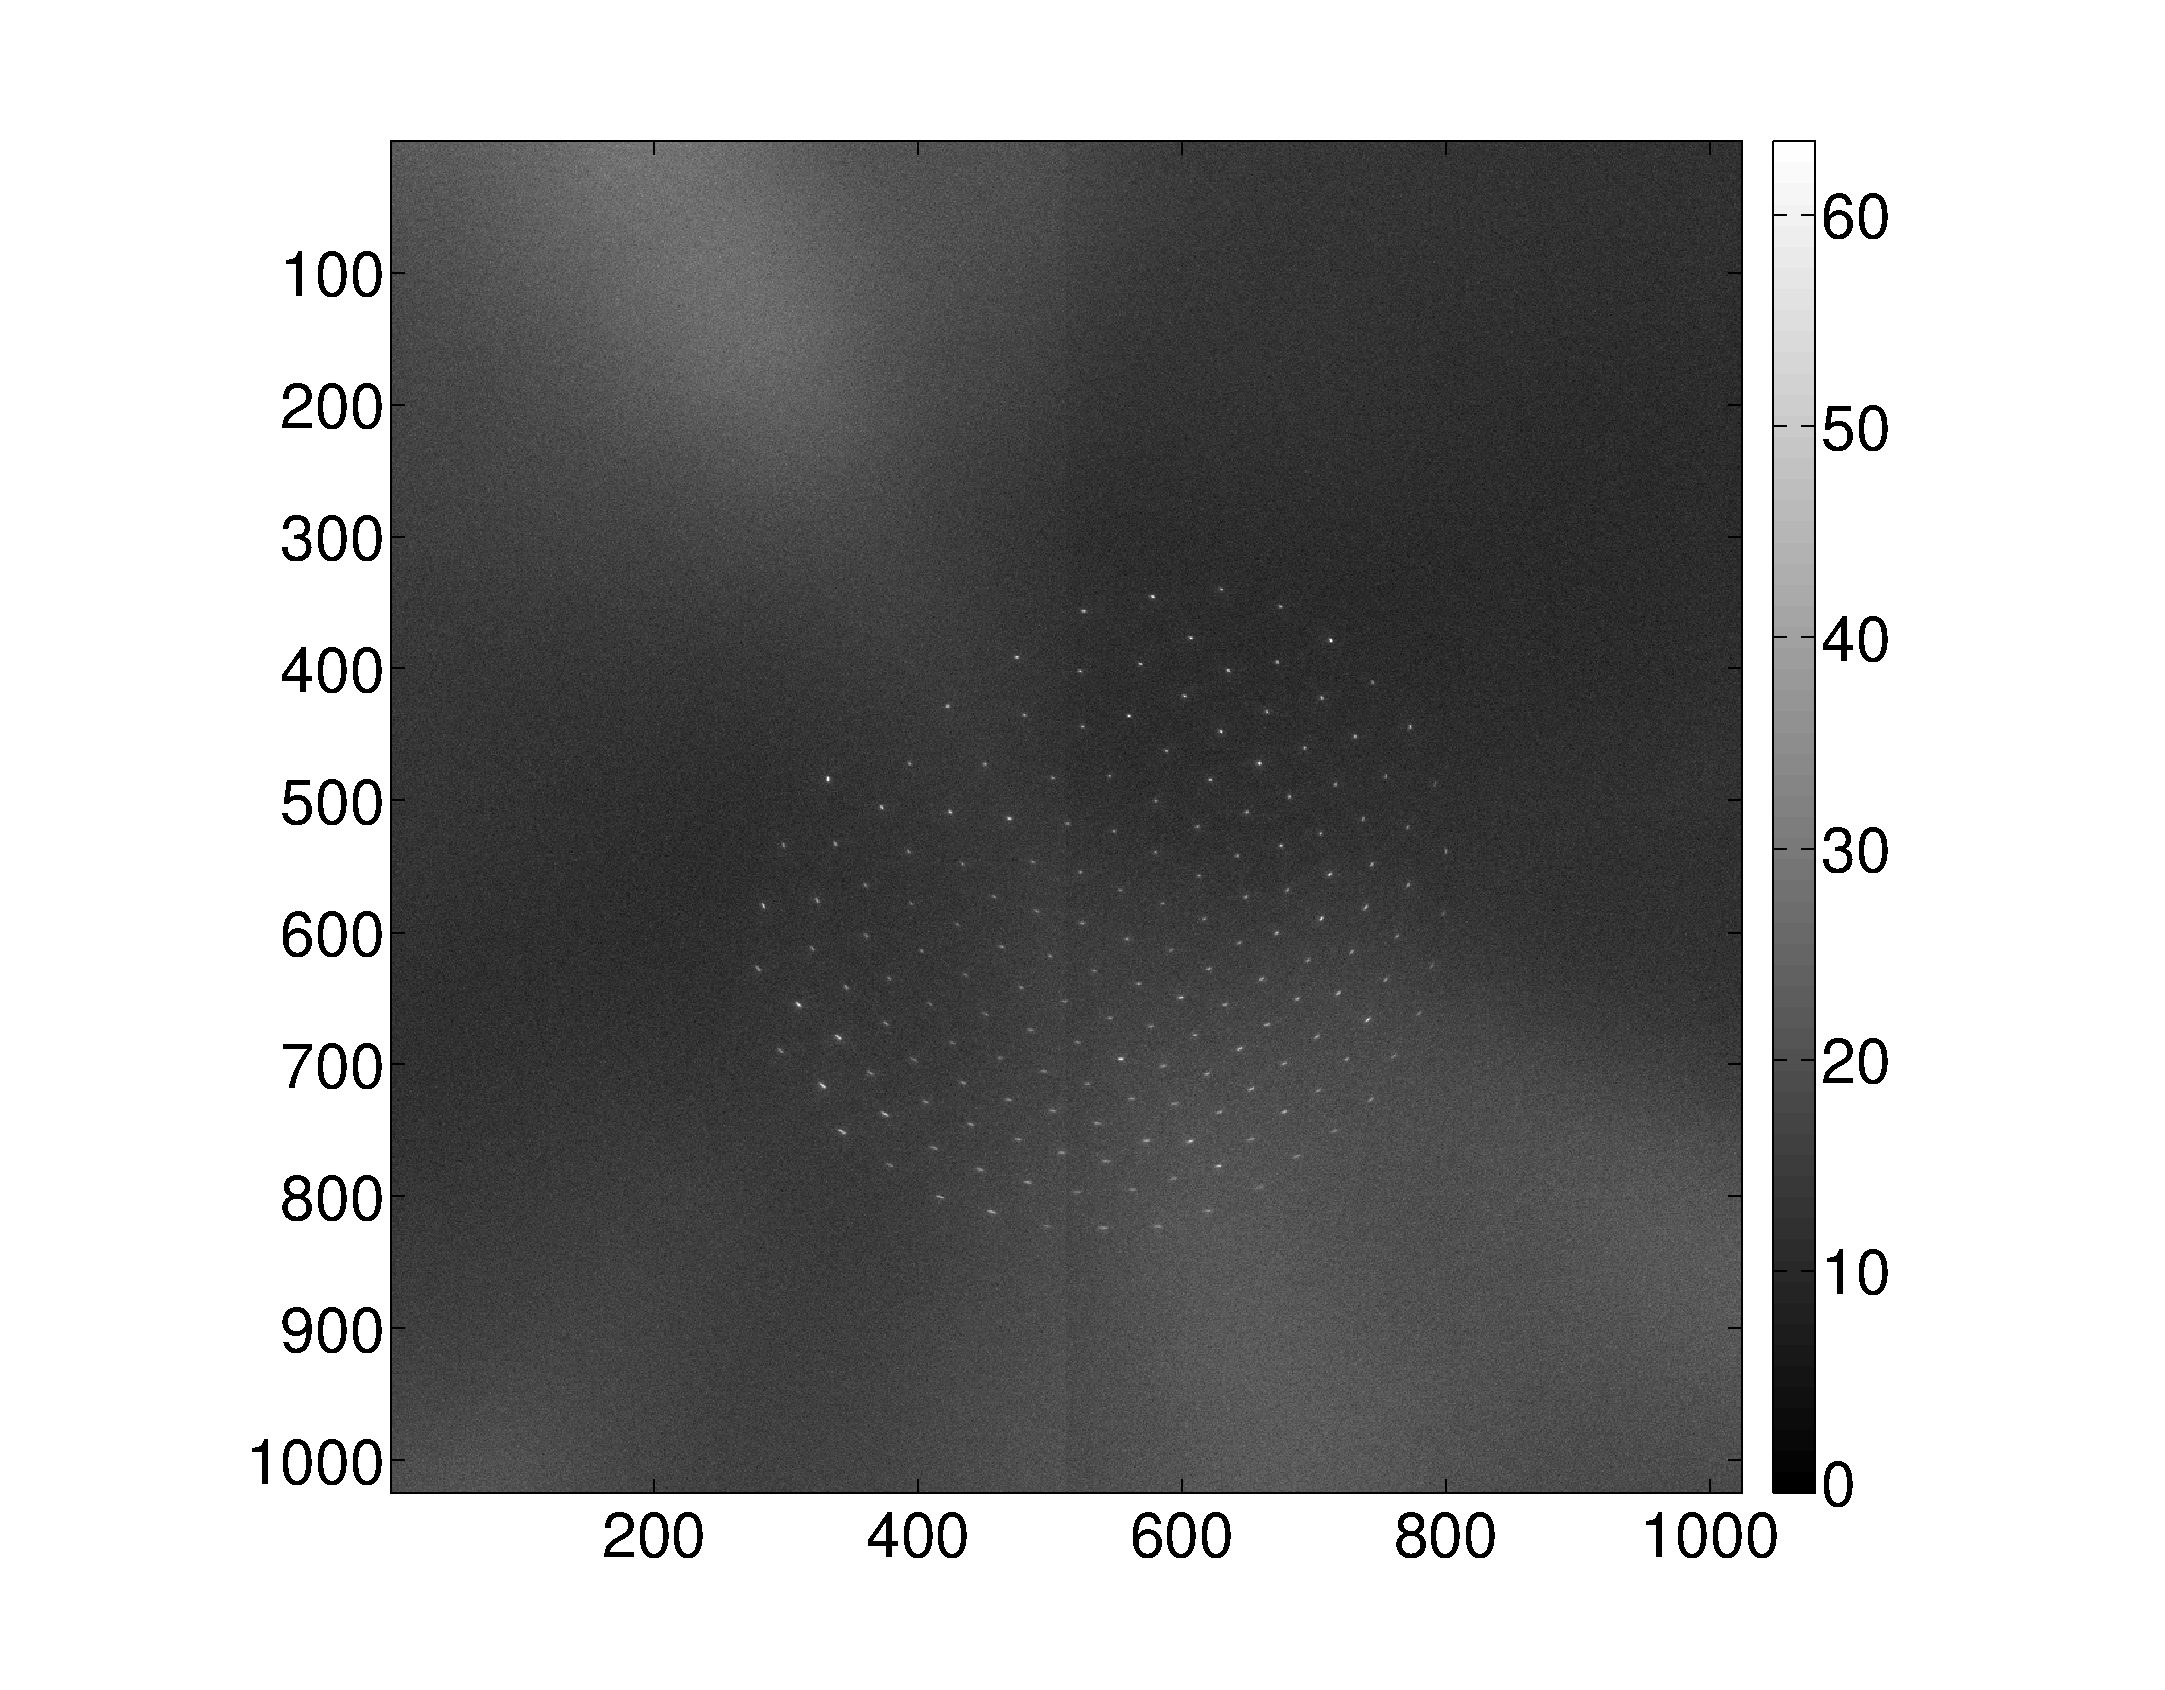
\includegraphics[width=0.95\columnwidth]{figures/eps/000000606627.eps}%
			\label{fig:forgo}
		}
		\caption{Két különböző kísérlet során készült fénykép.}
		\label{fig:captures}
	\end{figure}
	
	A fényképek alapján a részecskék pozíciójára és időbeli eloszlására vagyunk kíváncsiak.
	A kamera objektíve által leképezett kép a függőleges irányú pozíciót nem tartalmazza. Mivel jelen
	kísérletek során az ezirányú mozgása a részecskéknek nem számottevő, így az $x-y$ pozícióját jól
	lehet számítani a kép alapján. Nagy pontosság esetén szükséges a képek előzetes feldolgozása a
	perspektivikus torzítás kiküszöbölése végett. Természetesen ez lehetséges a pozíciók számítása után
	is, aminek a számításigénye kissebb is.




%----------------------------------------------------------------------------
\chapter{A részecskék detektálása}
%----------------------------------------------------------------------------

\section{Detektálási módszerek}
	A korábban látható \ref{fig:captures}. ábrán látható képeken kell a részecskéket felismerni és
	azoknak a koordinátáit exportálni.
	Erre több lehetőség adódik, amit a \cite{Feng2007} részletez.
	A detektáló módszereket a számítás igényeiknek növekvő sorrendjében mutatom be.
\subsection{Küszöb módszer}
	Legkézenfekvőbb módszer, hogy a kép pixeleinek világosságát összehasonlítjuk egy küszöb értékkel
	és ha az nagyobb ennél, akkor ezeket megjelöljük, mivel ott részecskét feltételezünk. 
	A módszer egyenletes háttér-világosság esetén jól működik és extra gyorsan számítható.
\subsection{Küszöb módszer szűréssel}
	A háttér világossága a \ref{fig:allo}. ábrán jól láthatóan nem egyenletes.
	A korábban említett egyszerű küszöb módszer itt nem alkalmazható, mivel a világos és sötét
	területek más és más küszöbértéket kívánnának meg.
	A megoldása erre, mint megannyi villamosmérnöki mérési feladatra, hogy a jel helyett a
	differenciális jelet mérjük. Jelen esetben ez azt jelenti, hogy először előállítjuk a részecske
	nélküli háttérképét, majd a méréssel kapott képből kivonva ezt a differenciális képet megkapjuk.
	A differenciális képen a részecskéket a korábban említett küszöb módszerrel lehet detektálni a
	részecskéket.
	
	Ehhez csupán a mérési képből kell szűréssel származtatni a háttérképet.
	A \cite{Feng2007,Oxtoby2010} cikkekben és általában erre véges Gauss szűrőt használnak, ami egy
	lineáris véges impulzusválaszú (FIR) aluláteresztő szűrő.
	A szűrés egy adott pixel környezetének súlyozott átlagolását jelenti.
	A súlyozás során szoroznunk kell, ami a bináris megvalósítás végett jóval lassabban történik, mint az
	összeadás avagy az összehasonlítás.
	
	Mivel a részecskék mérete a képen véges és kis szórású, így a korábban
	említett FIR Gauss szűrő jól tudja a részecskéket eliminálni.
	Viszont a mérési képek $100\ \mathrm{FPS}$ sebességgel és $1024\times1024$ mérettel érkeznek be.
	Ez $100\ \mathrm{MByte/s}$ adatfolyamot jelent. Ahhoz, hogy ezt közel online feltudjuk dolgozni a
	Gauss szűrés nem járható út. Hatékonyabb szűrőre van szükségünk! A megoldást a medián szűrőben látom,
	ami egy nemlineáris, de véges ``impulzusválaszú'' szűrő.
	A szűrő az adott pixel környezetének mediánjának számítását jelenti.
	A nemlinearitás jelen esetben nem okoz gondot, mivel csak detektálásra használjuk (a pozíció
	kinyerése az eredeti kép alapján készül, de ez később részletezve lesz.)
	
	A Gauss szűrő $n\times n$ környezet (ablak) esetén $n^2$ szorzást és $n^2-1$ összeadást jelent. Míg
	a medián szűrő $n\times n$ ablak esetén: bubborék rendezés során $O(n^2)$, javított bubborék
	rendezés során $O(n^2 / 2)$ illetve quicksort esetén $O(n\log n)$ összehasonlítást és
	cserét. Az összehasonlítás és a csere nagyságrendekkel gyorsabban végrehajtható, mint a szorzás és
	össeadás.
	
\subsection{Adaptív küszöb módszer szűréssel}
	Látható a \ref{fig:allo}. ábrán, hogy a sötétebb háttér kiterjedése nagyobb, ennek megfelelően az
	automata kamera ezekre a területekre állítja be az expozíciót.
	Így a sötét területek részletesebbek, míg a világos területek részletszegények (túlexponáltak) lesznek.
	Számunkra ez azt jelenti, hogy a sötétebb területeken jobban megbízhatunk a részecskék képében,
	míg a világosabb területeknél nem.
	Ezt a döntési küszöb értékének adaptációját jelenti a háttér világosságához.
	Az adaptív küszöböt a következő kifejezéssel határoztam meg:
	\begin{align} 
		\label{eq:treshold}
		K = \mathrm{Mean}\{\partial P\} + \delta \cdot \mathrm{STD}\{\partial P\} \cdot 
		\left[ 1+ a \left(
			\frac{\mhat{M}P}{\max\left\{\mhat{M}P\right\} - \min\left\{\mhat{M}P\right\}}
			\right)^b
		\right]
	\end{align} 
	ahol $P$ az eredeti kép, $\partial P$ a differenciális kép, $Mean\{\},\ STD\{\}$ az átlag és a
	szórás számításának függvénye, $\mhat{M}$ a medián szűrés operátora és $a,b$ két
	alakparaméter.\footnote{Az adaptív dontést a mérési kép előzetes feldolgozásával is elérhettük
	volna, ha a Photoshop-ból ismert Curves tool-al módosítottunk volna rajta.
	A tool a képet egy nemlineáris fügvényen keresztül engedi át.}
	
	A \ref{fig:alg}. ábrán látható a detektálási algoritmus működése közben.
	A \ref{fig:alg1}. ábrán a mérési kép ($P$) látható kitöltött görbével, ami az \ref{fig:allo}. ábrán
	látható mérési kép $x=40$ sora.
	Piros görbével látható a medián szűrt jelet ($\mhat{M}P$), amin jól érzékelhető a hirtelen
	változások eliminációja.
	A következő \ref{fig:alg2}. ábrán az eredeti és a szűrt különbsége azaz a differenciális kép
	($\partial P$) látható a kék görbével. A zöld görbe a \eqref{treshold} szerinti
	döntési köszöb.
	Az utolsó \ref{fig:alg3}. ábrán a detektált részecskék figyelhetőek meg.
	
	\begin{figure}[!h]
		\centering
		\subfloat[Eredeti (kitöltött) és a medián szűrt (folytonos) jel]{
			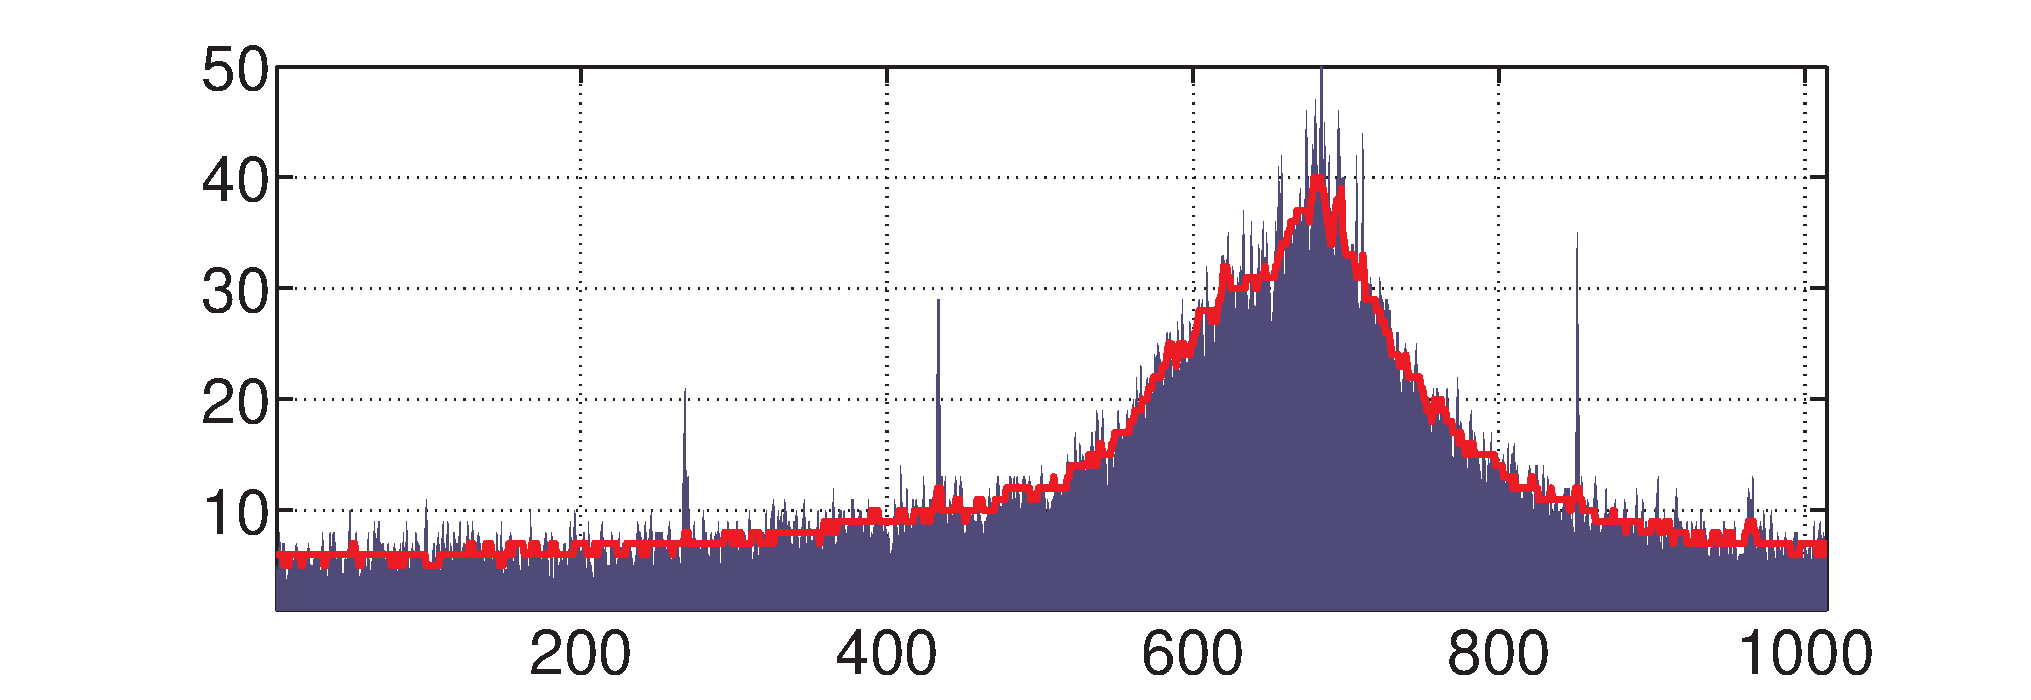
\includegraphics[width=0.95\columnwidth]{figures/eps/algoritmus1.eps}%
			\label{fig:alg1}
		}
		\\
		\subfloat[A differenciális jel (kék) és a döntési küszöb (zöld)]{
			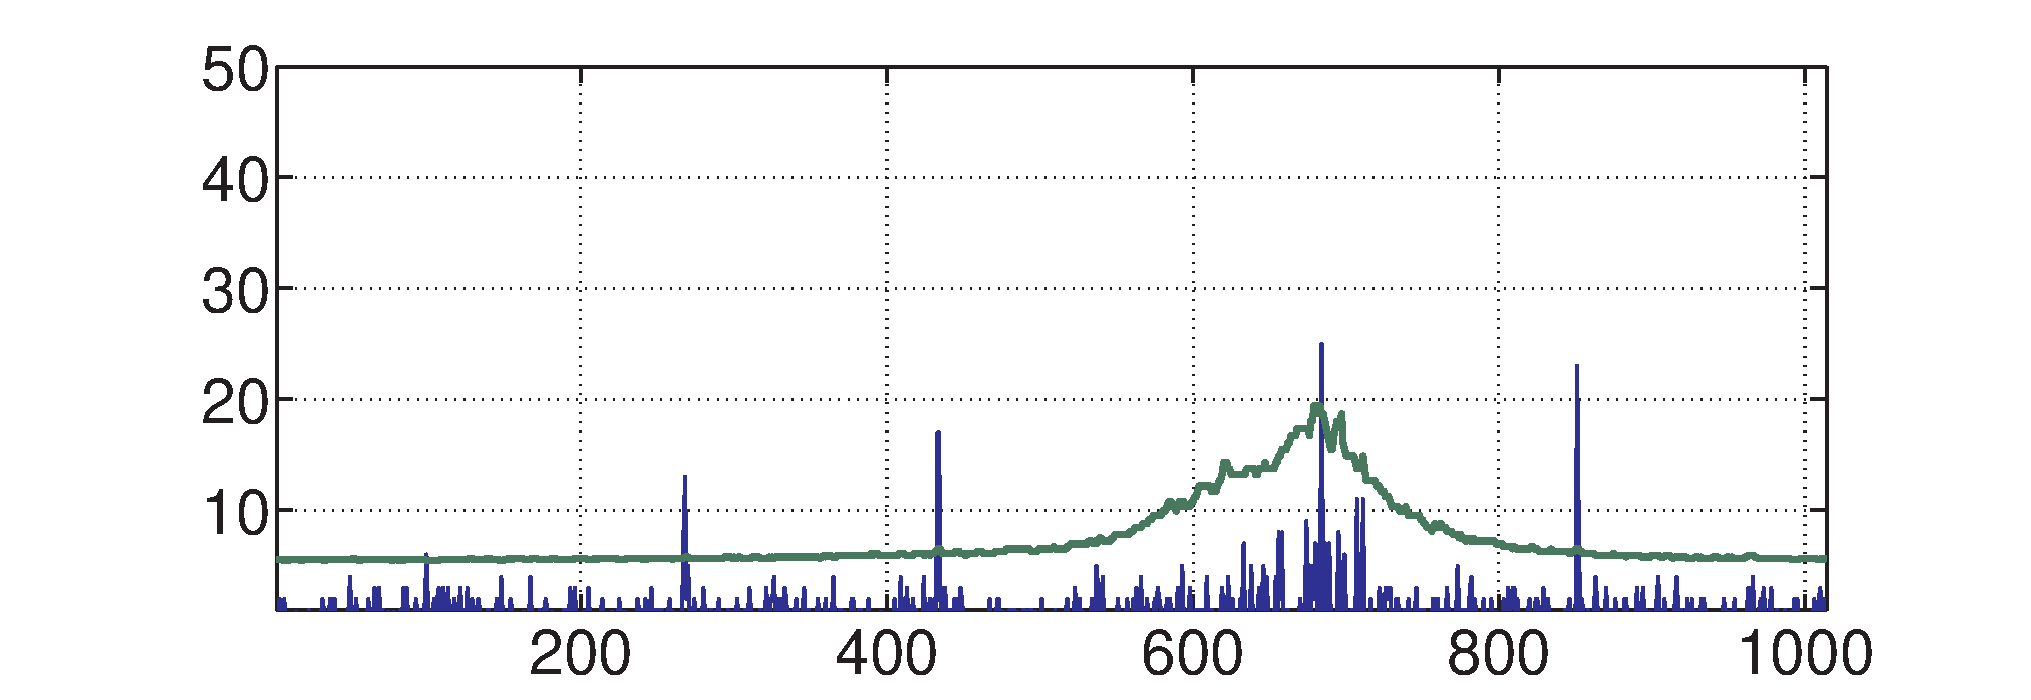
\includegraphics[width=0.95\columnwidth]{figures/eps/algoritmus2.eps}%
			\label{fig:alg2}
		}
		\\
		\subfloat[Detektált részecskék]{
			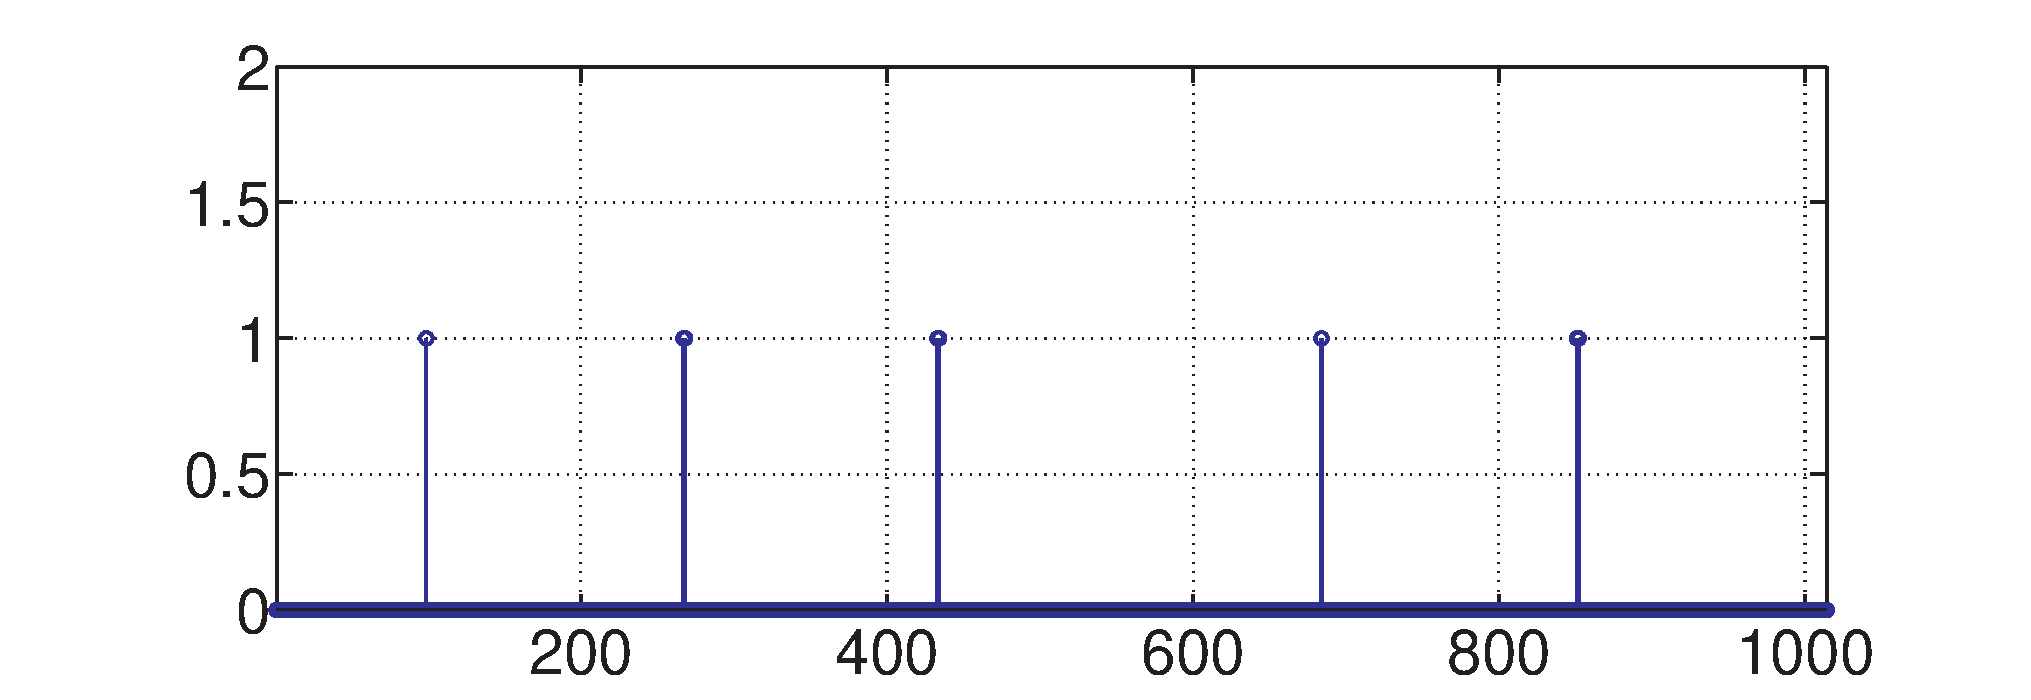
\includegraphics[width=0.95\columnwidth]{figures/eps/algoritmus3.eps}%
			\label{fig:alg3}
		}
		\caption[Adaptív küszöb bemutatása]{A medián szűrést alkalmazó adaptív küszöbbel részecskét
		detektáló algoritmus bemutatása az álló mérési kép (\ref{fig:allo}. ábra) $x=40$ során.}
		\label{fig:alg}
	\end{figure}
	
\section{A részecskék pozíciójának számítása}
	Kis felbontású kamera illetve nagyon kis porrészecskék esetén előállhat, hogy a részecskék egy
	pixelnyi területet foglalnak el a képen. Detektálás szempontjából ez kedvező viszont a pozíciómérés
	szempontjából nem, mivel ilyenkor a felbontásunk 1 pixelnyi. Ezen javítani a dithereléssel a
	következőképpen lehet: picit elállítjuk az élességet úgy, hogy egy részecske több pixel nagyságú
	``maszat'' legyen, majd a korábban részletezett detektálást elvégezzük.
	
	Ennek hatására egy részecske több pixelnyi felületet fog elfoglalni és a detektáló algiritmus is
	több pixelt fog megjelölni. A pozíció megtalálásához csoportosítani kell a megjelölt pixeleket.
	Az egy részecskéhez tartozó pixel-csoportot egy téglalap fogja határolni, amit region of
	interest-el (ROI) szokás illetni. Azonban a részecske detektálása után amorf formájú megjelölt
	pixeleink lesznek. Ezeket a könnyebb csoportosítás végett kiterjesztem pár pixellel az így kapott
	képet flood-fill algorimussal egybefüggővé teszem és ennek eredményeképp megkapom a ROI határoló
	koordiánáit, amit a következő két módszer felhasznál a részecske pozíciójának számítása során.
	\subsection*{Maximum keresés}
	Legegyszerűbb eset, ha a ROI-n belül az eredeti pixelek közül a legvilágosabbat veszem a
	részecske pozíciójaként.
	\subsection*{Szubpixel felbontás momentum módszerrel}
	Szofisztikáltabb, ha a ROI-n belül az eredeti pixelek világosságát, mint tömegpont tömegének veszem
	és a ROI-által határolt test súlypontját megkeresem. A módszerre kritikusan hat az előbb említett
	kiterjesztés mértéke. Ha túl nagy a kiterjesztés, akkor azzal hibát viszek be pozicíó mérésébe,
	míg ha túl kicsi akkor meg egy részecskének akár két képe/pozíciója keletkezhet.
	
	\noindent Az algoritmus hatékonyságát különböző $\delta$ érték mellett a következő \figref{roi}
	ábrán látható.
	
	\begin{figure}[H]
		\centering
		\subfloat[$\delta = 10$]{
			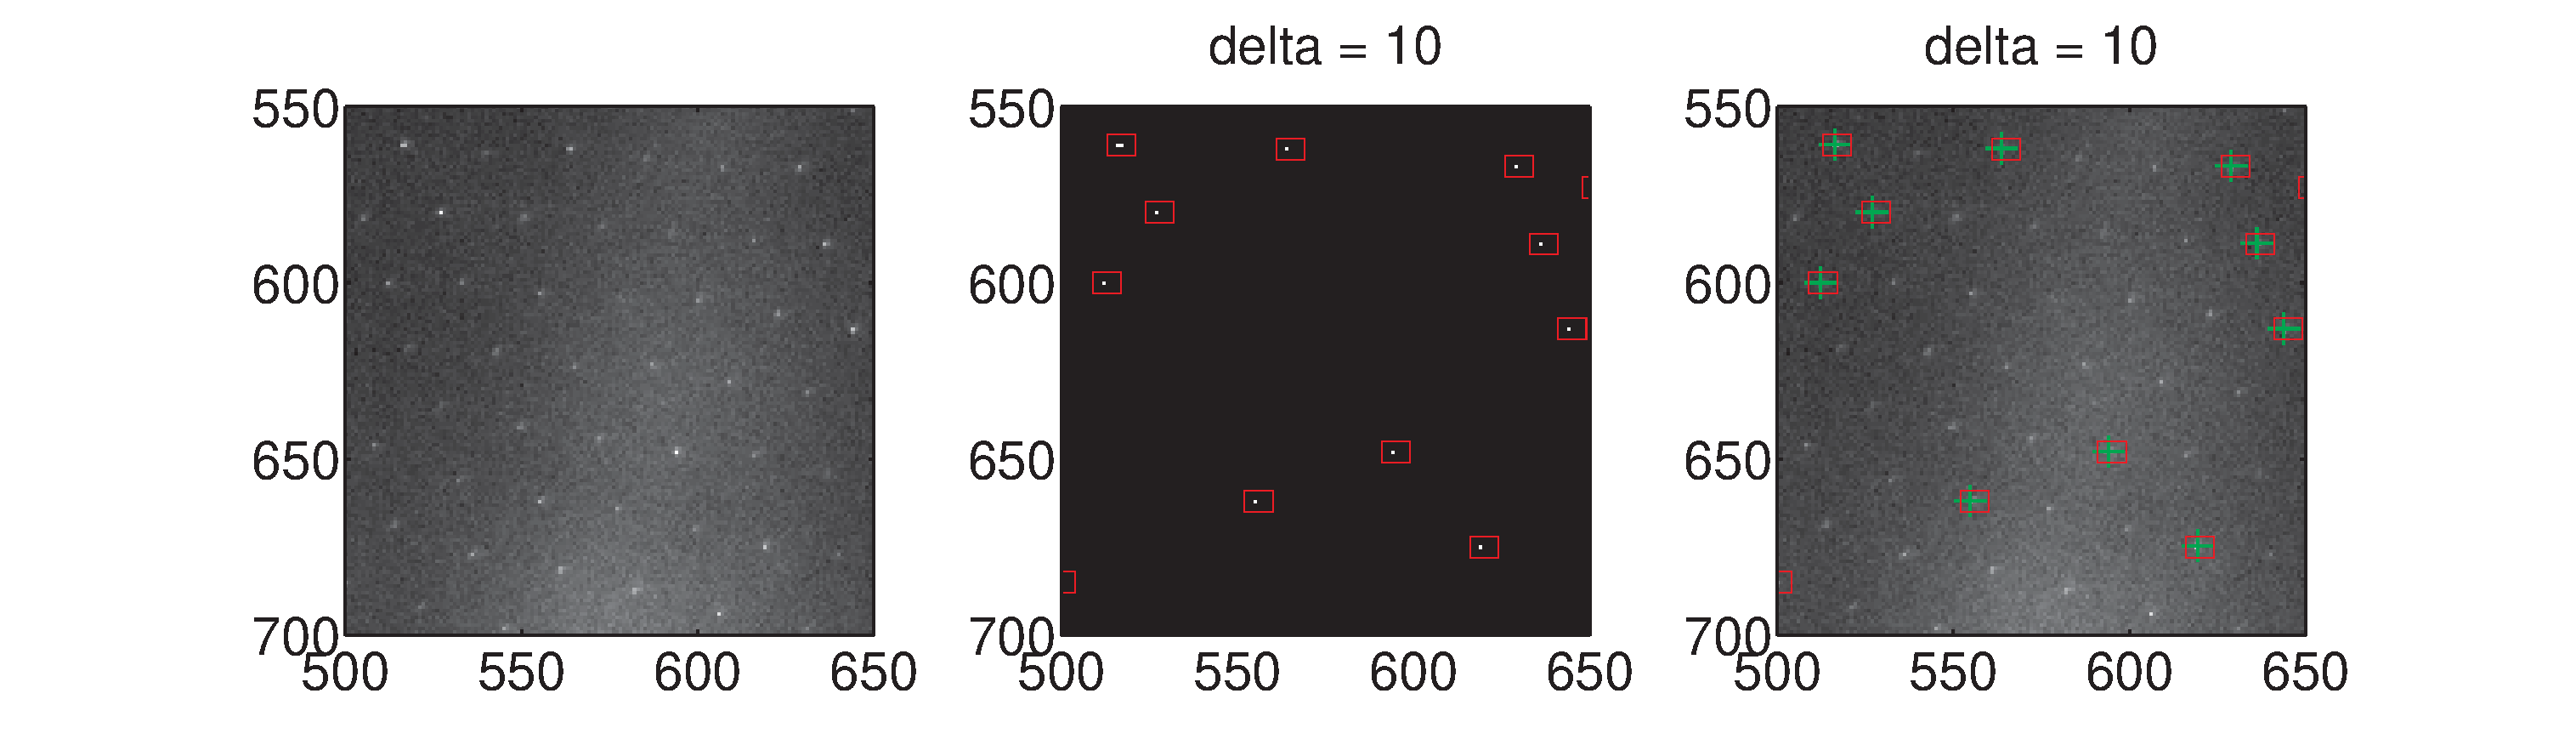
\includegraphics[width=1\columnwidth]{figures/eps/delta10.eps}%
			\label{fig:delta4}
		}
		\\
		\subfloat[$\delta = 2$]{
			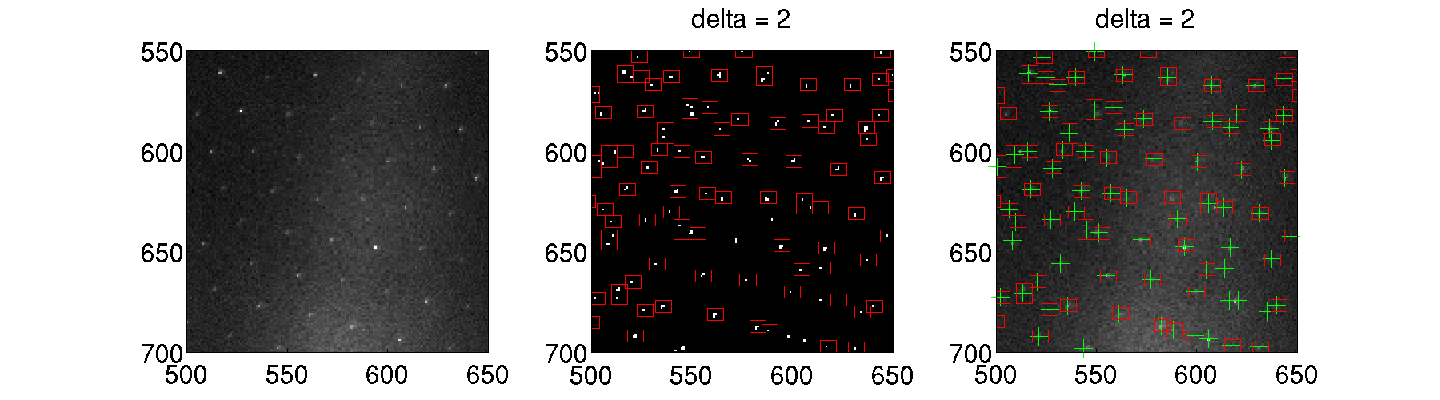
\includegraphics[width=1\columnwidth]{figures/eps/delta2.eps}%
			\label{fig:alg3}
		}
		\\
		\subfloat[Optimális $\delta = 3.5$]{
			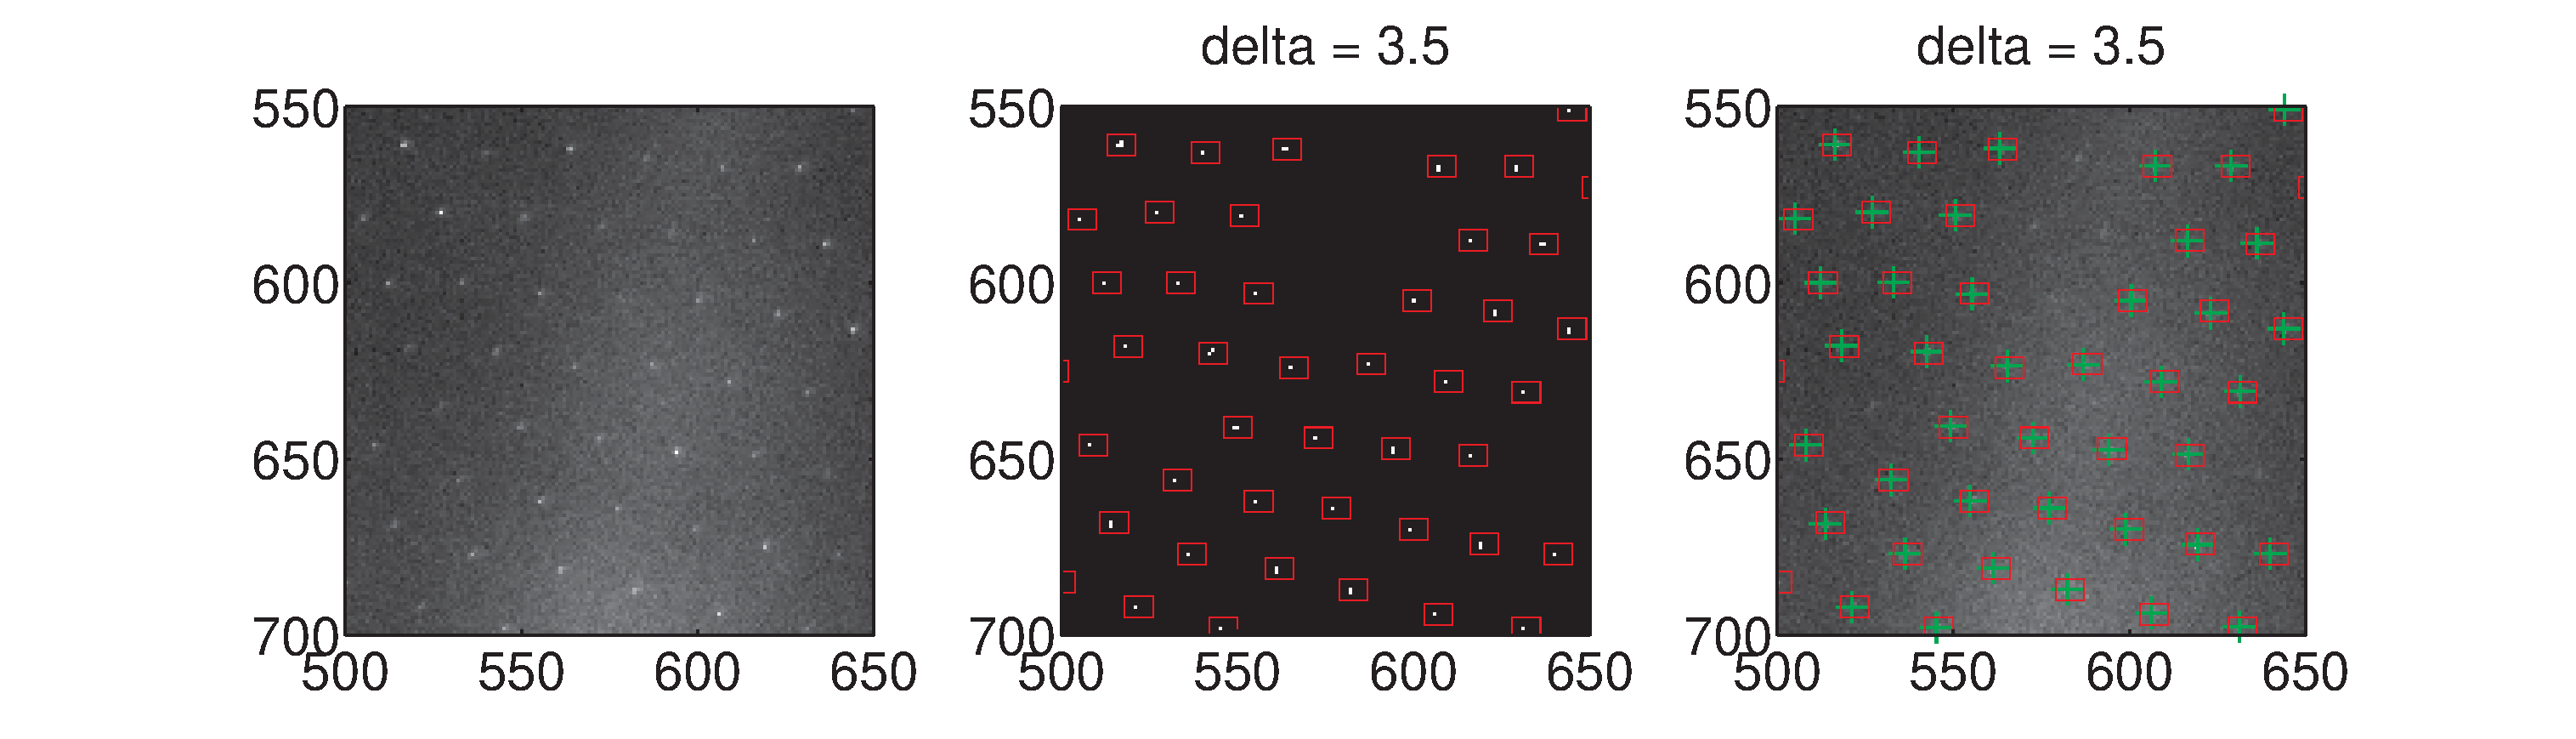
\includegraphics[width=1\columnwidth]{figures/eps/deltaopt.eps}%
			\label{fig:deltaopt}
		}
		\caption[Pozíciómérés momentum módszerrel]{Az adaptív küszöb módszerrel detektált részecskék
		momentum módszerrel számított pozíciója. \textbf{Bal oszlopban} az eredeti mérési kép, \textbf{középső oszlopban} a detektálás
		eredménye és a ROI, az \textbf{utolsó oszlopban} az eredeti mérési képen a ROI és a detektált
		részecske pozícióját jelző kereszt.}
		\label{fig:roi}
	\end{figure}
	
	\noindent
	\begin{center}
	Az algoritmus jól párhuzamosítható, ami a nagyteljesítményű multiprocesszoros
	környezetben kedvező futási időt eredményezhet. A párhuzamos program létrehozásának segítségére az 
	OpenCL keretrendszert választottam, aminek a bemutatása következik.
	\end{center}






%----------------------------------------------------------------------------
\chapter{A multiprocesszoros OpenCL környezet} \label{sec:opencl}
%----------------------------------------------------------------------------

\section{OpenCL architektúrája}
	Az Open Computing Language (OpenCL) keretrendszer \cite{opencl}
	általános modellt, magas szintű programozási interfészt és hardware
	absztrakciót nyújt a fejlesztőknek adat- vagy feladat párhuzamos számítások gyorsítására különböző
	számítóegységen (CPU, GPU, FPGA, DSP, \ldots).
	A hárdvergyártók implementálják az OpenCL szabványt, ami által saját platformot
	hoznak létre. Egy ilyen platformon belüli eszközök alatt főként GPU-kat, de
	CPU-kat és FPGA-t \ldots is értünk.
	OpenCL keretrendszerben történő programozás során két programot kell írnunk.
	Az egyik a kernel, ami az eszközön futatott szálra fog leképeződni.
	A másik a gazda processzoron (host-on) futó host-program, ami elvégzi az I/O műveleteket,
	a probléma összeállítását, a memória allokálást, az argumentumok beállítását
	illetve a kernel meghívását az eszközön.
	A kernel futása végeztével a host-program kiolvassa az eszközből
	a kívánt eredményt.
	
	\begin{figure}[!ht]
		\centering
		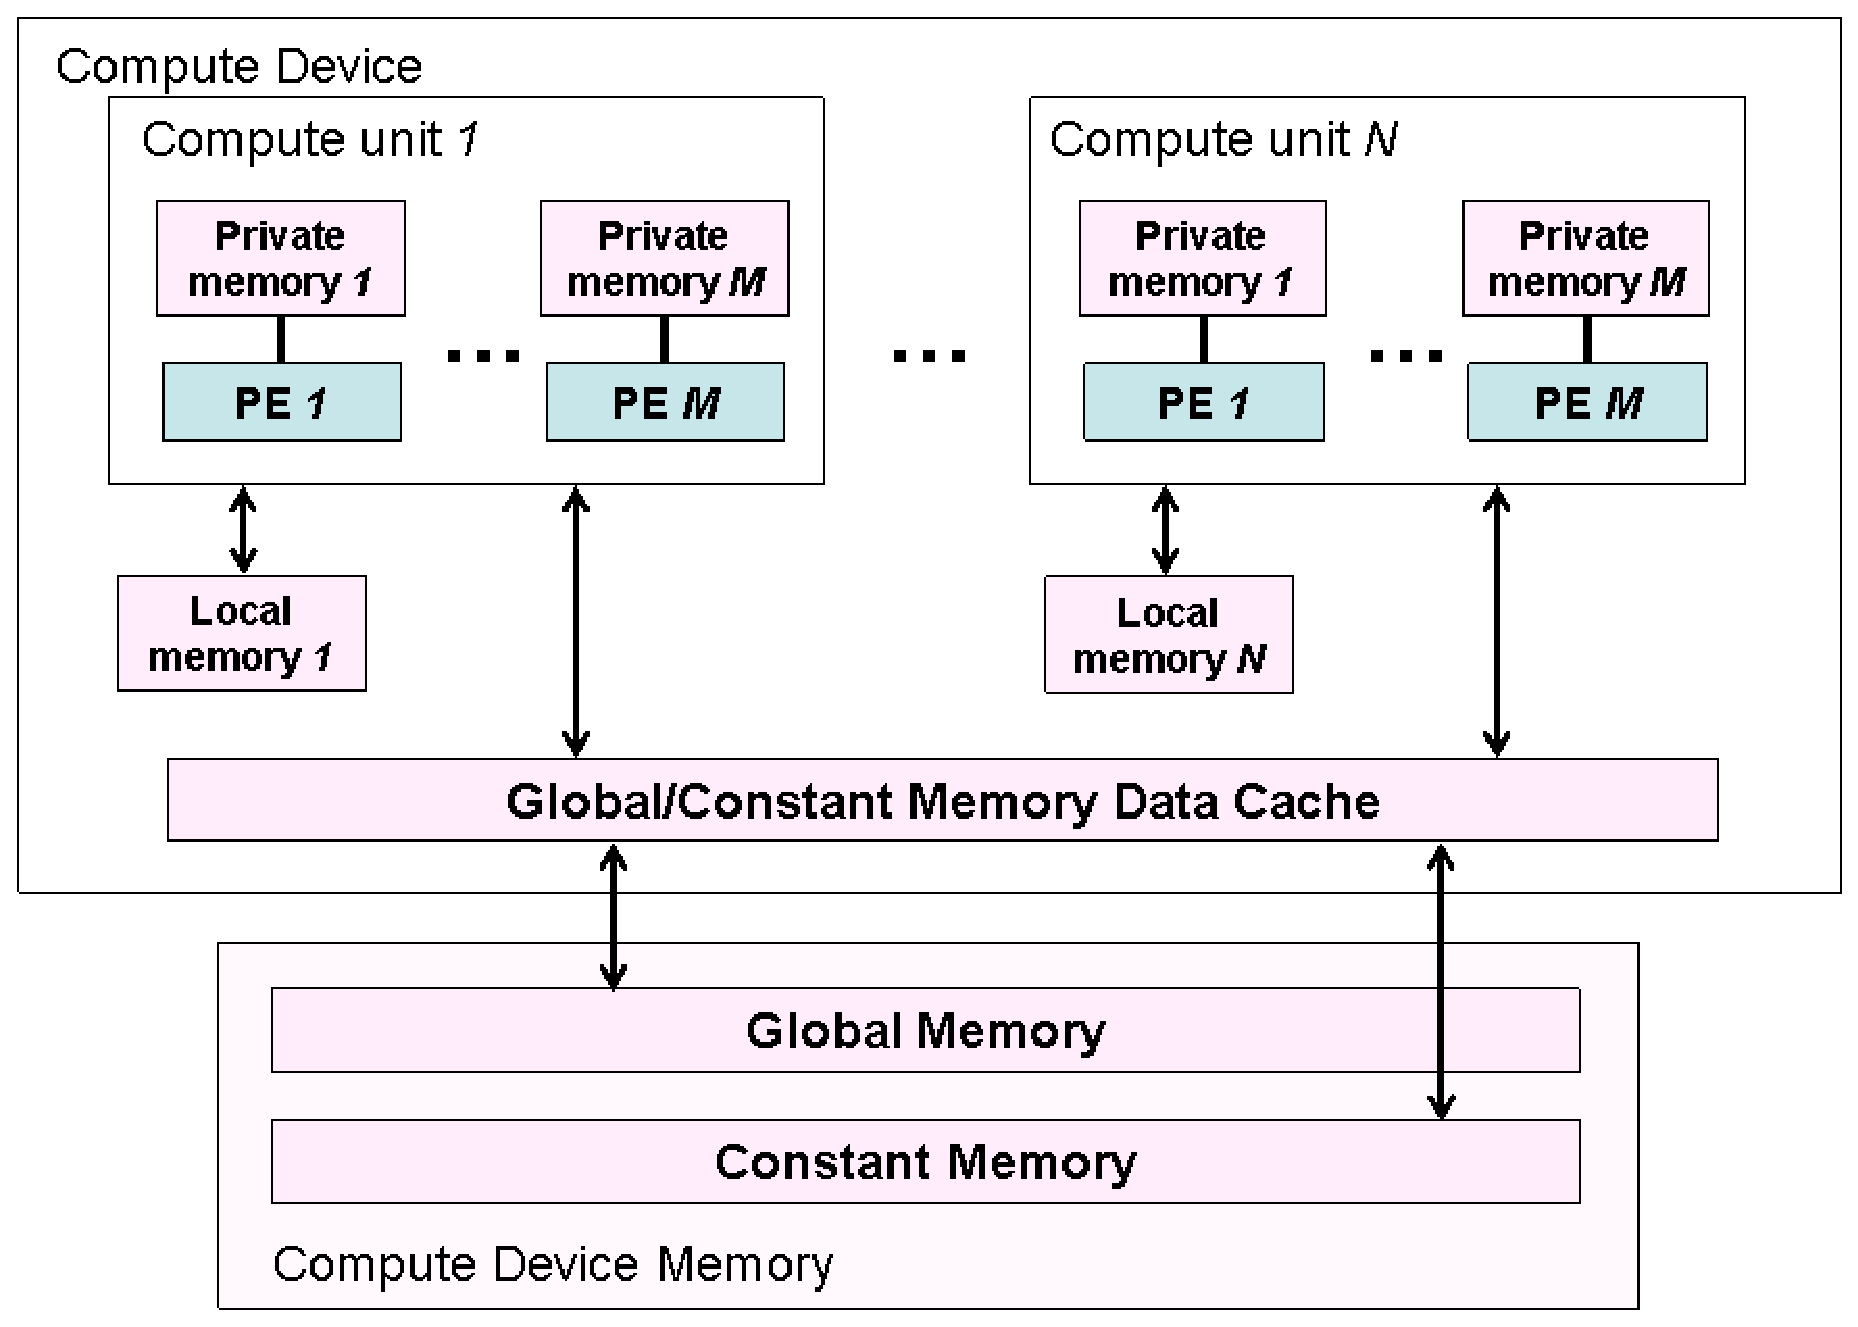
\includegraphics[width=0.6\columnwidth]{figures/eps/device.eps}
		\caption{OpenCL device architektúra (forrás: \cite{opencl})} 
		\label{fig:device} 
	\end{figure}
	Az eszközök multiprocesszoros architektúrával és ezek kiszolgálására képes
	memória architektúrával rendelkeznek, amit a \ref{fig:device} ábra vázol.
	Egy eszköz több compute unit-ot (processzor-magot) tartalmaz.
	Az OpenCL négy memória szintet különböztet meg, amikre a
	következőképpen hivatkozik:
	\begin{itemize}
		\item \emph{Regiszterek:} Private memory,
		\item \emph{Chipen belüli memória (cache):} Local memory,
		\item \emph{Chipen kívüli memória:} Global memory és Constant Memory.
	\end{itemize}
	A regiszterek és lokális memória kis méretűnek és gyors elérésűnek mondható, míg
	a globális memória nagynak, de lassú elérésűnek.
	A memóriákra megkötésként szolgál, hogy ki allokálhat, írhat és olvashat
	belőle. A \ref{table:mem}. táblázatban látható ezen jogosultságok.
	\begin{table}[!h]
	%\renewcommand{\arraystretch}{1.3}
	% if using array.sty, it might be a good idea to tweak the value of
	% \extrarowheight as needed to properly center the text within the cells
	\caption{OpenCL memória szintek}
	\label{table:mem}
	\centering
	% Some packages, such as MDW tools, offer better commands for making tables
	% than the plain LaTeX2e tabular which is used here.
	\begin{tabular}{l|l|l|l|l}
			 & Global memory & Constant mem. & Local mem. & Private mem.\\ \hline
		Host & Dinamikusan R/W & Din. R/W & Din. R/W & \\
		Kernel & R/W & Statikusan R & Satik. R/W & Statik. R/W\\
		Sebesség & Lassú & Gyors & Gyors & Regiszter\\
		Méret & $1$ Gbyte $<$ & $\sim64$ Kbyte& $\sim16$ Kbyte & $<1$ Kbyte
	\end{tabular}
	\end{table}
	
	Ahhoz, hogy a rendszerben rejlő teljesítményt kihozzuk három fontos kérdést
	kell a szimulátor magjának implementálásakor megválaszolnunk:
	\begin{itemize}
		\item \emph{Mennyit?} Tisztában kell lennünk az aktuális
		memória fogyasztással és a szükséges memóriamérettel.
		\item \emph{Honnan-hova?} Fontos, hogy a lehető legközelebb legyen az adat
		a processzor-maghoz.
		\item \emph{Mikor?} Mivel a memória művelet alatt a futtatott kernel nem
		dolgozik, így átadja a helyét egy másiknak. (Ez Direct Memory Access (DMA)
		blokk létezése allatt igaz). Ennek a megfelelő szinkronizációjával nagyobb
		kihasználtság érhető el (load balance).
	\end{itemize}
	
	
\section{OpenCL programozási modell}
	
	A programozási modell középpontjában a kontextus áll, ami az OpenCL
	osztálydiagrammján (\ref{fig:class}. ábra) figyelhető meg.
	A futtatáshoz szükséges, hogy a kontextushoz platformot, majd azon belül
	eszközt, az eszközhöz programot (kernelt) és memóriát rendeljünk.
	\begin{figure}[!ht]
		\centering
		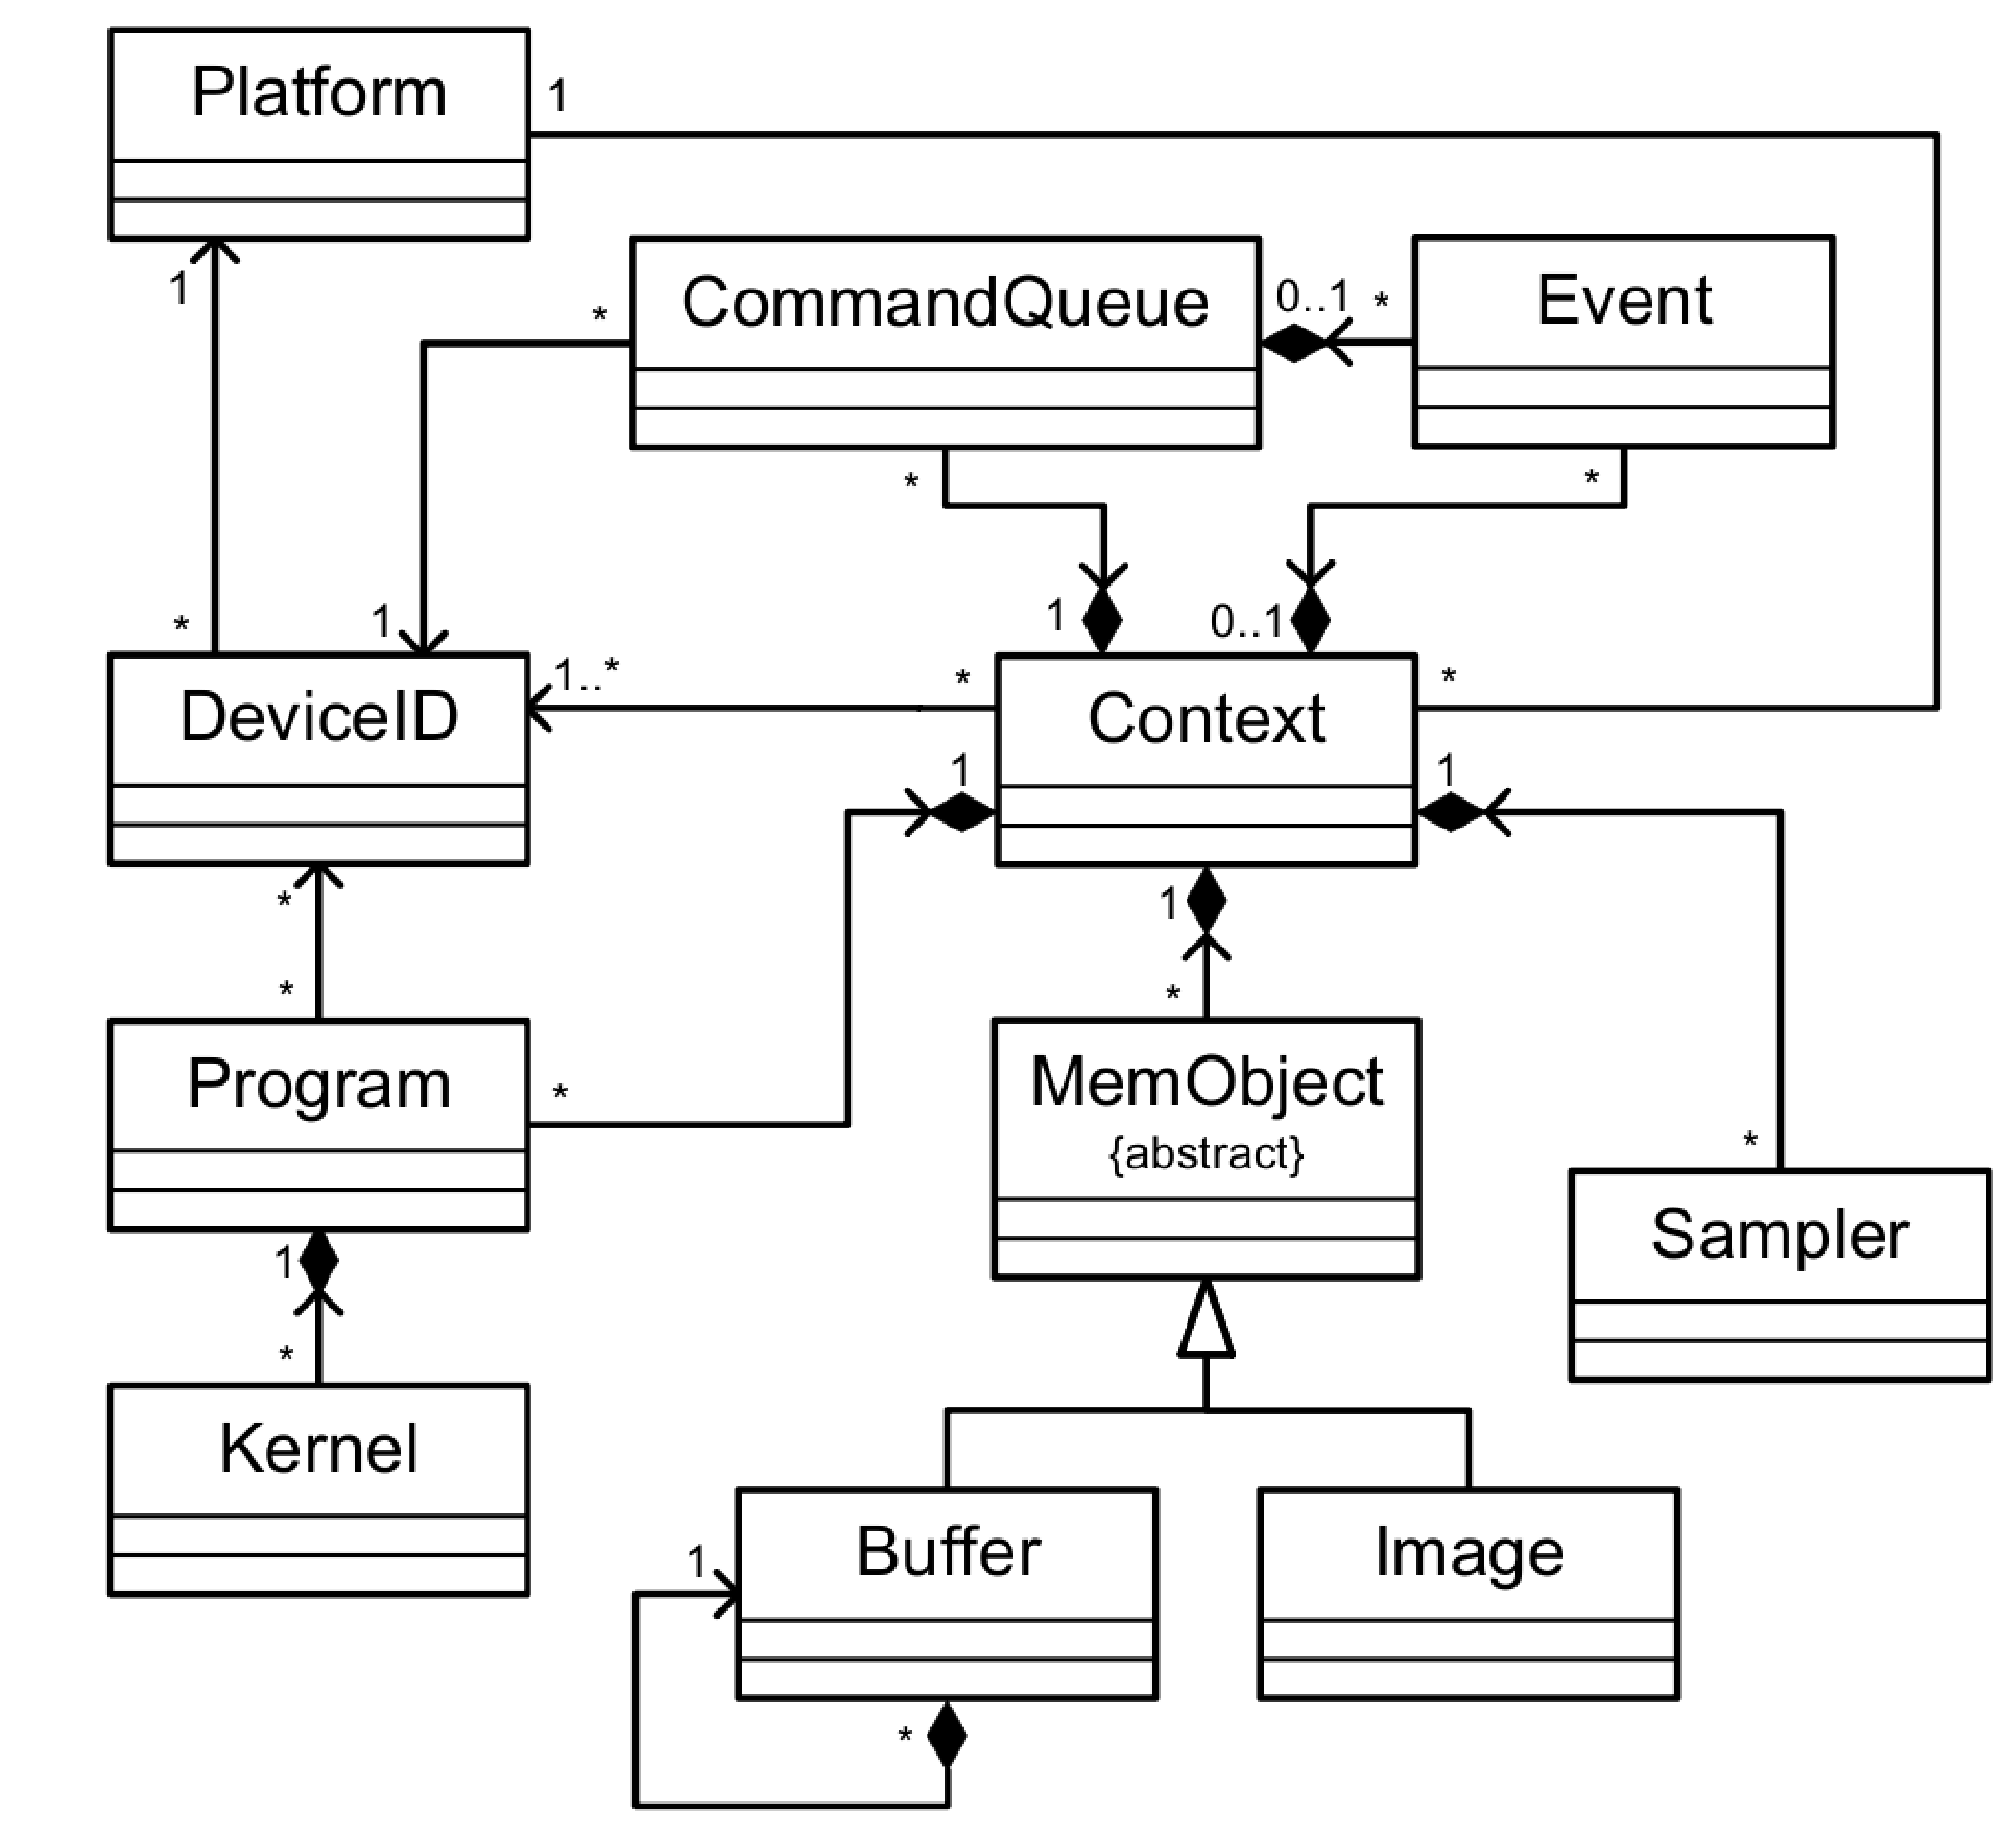
\includegraphics[width=0.6\columnwidth]{figures/eps/context.eps}
		\caption{OpenCL context osztálydiagrammja (forrás: \cite{opencl})} 
		\label{fig:class} 
	\end{figure}
	Figyelembe kell vennünk azt a megkötést, hogy csak az egy platformon belüli
	eszközök programozhatóak heterogén módon. Például: Intel platform esetén
	lehetséges CPU-t, processzorkártyát és Intel-es GPU-t programozni.
	
	A programozással megoldandó problémát kétféleképpen lehetséges a feldolgozó
	egységekhez (work-item) avagy processzorokhoz rendelni:
	adat parallel módon vagy taszk parallel módon.
	
	Adat parallel módon (\ref{fig:data_parallel} ábra) a feldolgozandó adat egy
	részéhez rendelünk egy feldolgozó egységet. Fontos figyelembe venni az eszköz korlátos
	számú feldolgozó egységének számát. Ha nem elég a feldolgozó egysége akkor a
	feladat megfelelő partícionálásával lehetséges kordában tartani a szükséges
	erőforrás számát.
	
	Taszk parallel módot (\ref{fig:task_parallel} ábra) olyan esetben célszerű
	használna, ha a bemenet dinamikus mérete a futási időben rendkívül változik
	illetve a végrehajtandó feladat lazán függenek össze.
	
	\begin{figure*}[!ht]
		\centering
		\subfloat[Adat parallel]{
			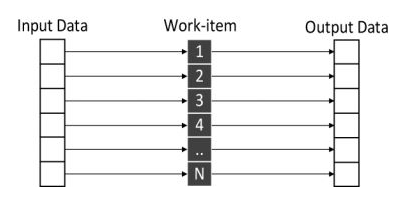
\includegraphics[width=0.45\columnwidth]{figures/eps/data.eps}%
			\label{fig:data_parallel}
		}
		\hfil
		\subfloat[Taszk parallel]{
			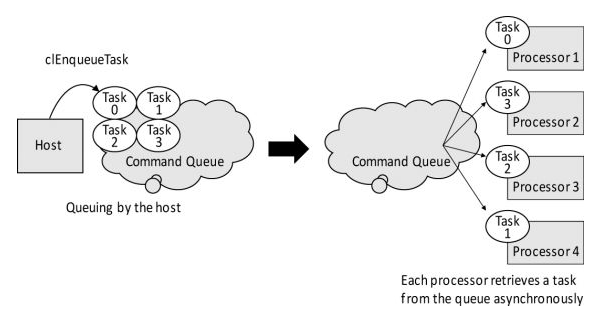
\includegraphics[width=0.45\columnwidth]{figures/eps/task.eps}%
			\label{fig:task_parallel}
		}
		\caption{Feladat hozzárendelése work-item-hez (processzorhoz)}
		\label{fig:parallel}
	\end{figure*}
	A processzor-magok megfelelő kihasználtságának elérése végett több ezer
	work-item virtuálisan osztozik rajta.
	Továbbá ezen work-item-eket work-group-okba rendezzük.
	
	A work-itemeket jelen pillanatban az OpenCL specifikációja \cite{opencl} szerint 3 dimenziós
	work-group-ba tudjuk rendezni. Egy példát láthatunk egy work-item indexének a globális és lokális megfelelőjére a
	követekző \ref{fig:ndrange}. ábrán.
	
	\begin{figure}[!h]
		\centering
		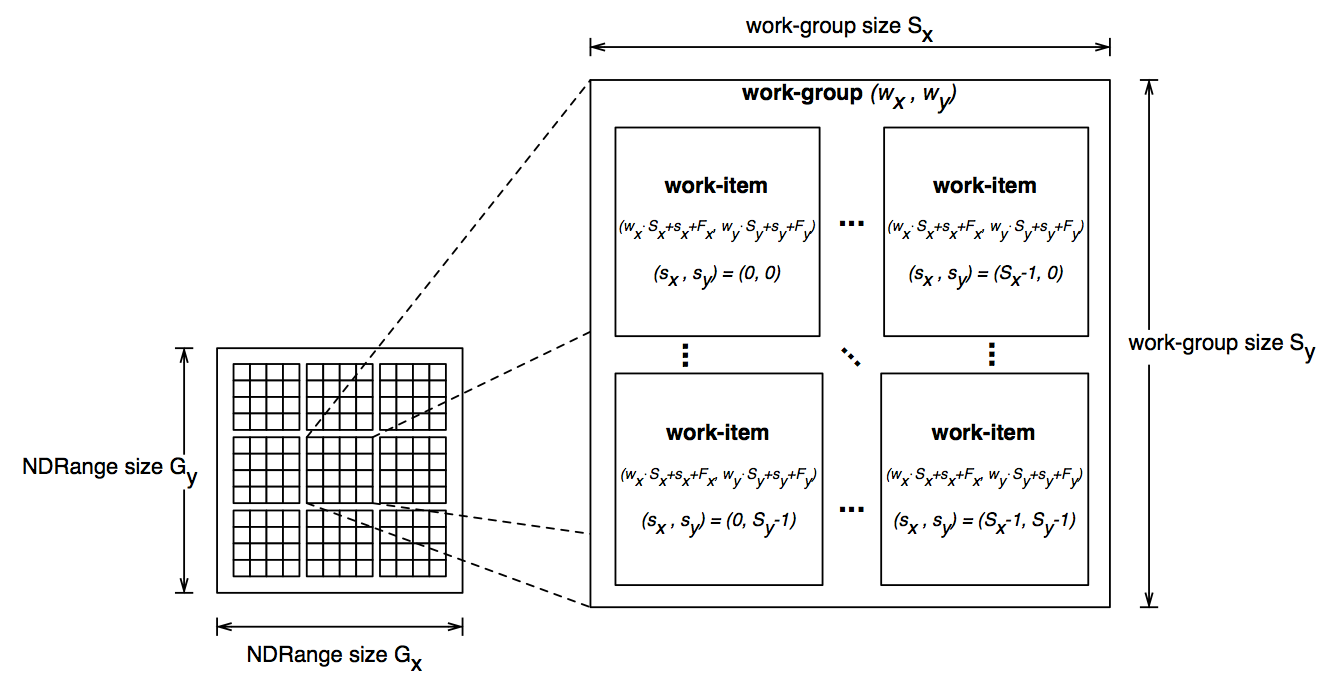
\includegraphics[width=0.9\columnwidth]{figures/eps/ndrange.eps}
		\caption{2D-s work-item-ek work-group-ba rendezése és indexelése (forrás: \cite{opencl})} 
		\label{fig:ndrange} 
	\end{figure}

	A work-group-okba rendezés a lokális memória jogusultsága miatt érdekes.
	Konkrétan az egy work-group-ba tartozó összes work-item azonos lokális memórián
	osztozik.
	Ennek a következménye az, hogy adat parallel módú feldolgozás esetén
	az egymásra ható adatokhoz tartozó work-item-eket egy work groupba kell
	rendelnünk.
	Ha ez nem lehetséges, akkor a globális memóriához kell fordulnunk.
	A globális memória avagy a bank szervezésű külső (off-chip) memóriák
	hozzáférési ideje relatíve nagy így ezek használatát lehetőleg el kell kerülni
	és a programozónak kell ``cachelni" a lokális memóriába.
	
	Mivel a work-item-ek konkurrensen hajtódnak végre, így az általuk közösen elérhető memóriákra
	(globális, lokális) nézve versenyhelyzetben vannak.
	Az OpenCL ezt a problémát a laza memóriamodell használatával oldja meg. Az alkalmazott
	szinkronizáció egy korlátot tesz a programban, amit csak akkor léphet át, ha az összes többi
	work-item az azonos work-group-ban ezta a korlátot már elérte. Erre a \texttt{barrier(FLAG)}
	függvényhívás szolgál. Fontos megjegyezni, hogy ez a szinkronizáció csak egy adott
	work-group-on belül történik, a work-group-ok közötti szinkronizációra nincs lehetőség. 
	
	\begin{center}
	Összefoglalva: nagy hangsúlyt kell a memóriaszervezésre fordítani, hogy a
	processzormagok megfelelően legyenek az adatokkal táplálva.
	\end{center}


\section{Futási környezet bemutatása}
	A következő eszközök teljesítményét vizsgálom:
	\begin{itemize}
		\item A laptopomban található \textbf{Intel Core i5 M520} processzor,
		\item A laptopomban található kis teljesítményű \textbf{nVidia GT330M} videókártya,
% 		\item Asztali PC-ben található \textbf{Intel Xeon CPU},
% 		\item Asztali PC-ben található \textbf{Intel Xeon Phi} co-processzor \cite{phi,mic}. 
	\end{itemize}
	Ezen eszközök legjelentősebb paraméterei a \ref{table:envs} táblázat tartalmazza.
	
	\begin{table}[!ht]
	%\renewcommand{\arraystretch}{1.3}
	% if using array.sty, it might be a good idea to tweak the value of
	% \extrarowheight  as needed to properly center the text within the cells
	\setlength{\extrarowheight}{8pt}
	\caption{Használandó eszközök összehasonlítása}
	\label{table:envs}
	\centering
	\footnotesize
	% Some packages, such as MDW tools, offer better commands for making tables
	% than the plain LaTeX2e tabular which is used here.
% 	\begin{tabular}{ l | r | r | r | r}
% 		 & Intel Core i5 & nVidia GT330M & Intel Xeon & Xeon PHI \\ \hline
% 		MAX COMPUTE UNITS & $4$ & $6$ & $8$ & $224$\\
% 		MAX CLOCK FREQUENCY & 2400 & 1265 & 3000 & 1100\\
% 		MAX WORK GROUP\_SIZE & $8192$ & $512$ & $8192$ & $8192$ \\ \hline\hline
% 		GLOBAL MEM SIZE & $\sim 4Gbyte$ & $1Gbyte$ & $8Gbyte$ & $\sim 4.5Gbyte$\\
% 		%MAX\_CONSTANT\_BUFFER\_SIZE & $131072$ & $65536$ & $131072$ & $131072$\\
% 		LOCAL MEM SIZE & $32 Kbyte$ & $16 Kbyte$ & $32 Kbyte$ & $32 Kbyte$\\
% 	\end{tabular}
	
	\begin{tabular}{ l | r | r}
		 & Intel Core i5 M520 & nVidia GT330M \\ \hline
		MAX COMPUTE UNITS & $4$ & $6$\\
		MAX CLOCK FREQUENCY & 2400 & 1265 \\
		MAX WORK GROUP\_SIZE & $8192$ & $512$ \\ \hline\hline
		GLOBAL MEM SIZE & $\sim 4Gbyte$ & $1Gbyte$\\
		%MAX\_CONSTANT\_BUFFER\_SIZE & $131072$ & $65536$ & $131072$ & $131072$\\
		LOCAL MEM SIZE & $32 Kbyte$ & $16 Kbyte$\\
	\end{tabular}
	\end{table}
	
	Az összehasonlíthatóság végett a legkissebb memóriájú eszközre fogom a problémát skálázni, ami a
	GT330M videókártya. A többi eszköz memóriája jóval nagyobb, így a kód mindegyiken tud futni.





%----------------------------------------------------------------------------
\chapter{Fejlesztőkörnyezet összeállítása}
%----------------------------------------------------------------------------

	OpenCL kód fejlesztése történhet Windows alatt NVIDIA Nsight Visual Studio
	Edition \cite{nsight} és Linux alatt GCC-vel \cite{gcc}.
	Az Open Source fejlesztőrendszer ingyenessége és az általa generált program hordozhatósága végett
	a Linux alatti fejlesztés mellett döntöttem. 
	Az OpenCL-t támogató hardverek legtöbbször CPU-k, GPU-k és az Intel MIC
	\cite{mic} kártyái.
	Ezekre való OpenCL kód fejlesztéséhez a gyártók biztosítanak Software Developement Kit-et (SDK).
	Ezek telepítése szinte bármelyik Linux disztribúción sikerülhet a megfelelő követelmények előzetes telepítése után.
	A Linux diszrók közül a CentOS-re \cite{centos} esett a választás, ami 
	csupán a fejlesztőkörnyezet egyszerűbb telepítése végett történt így.

\section{Software Developement Kit-ek (SDK) telepítése} \label{sect:sdk}
\subsection{nVidia támogatás telepítése}
	A legtöbb mai Linux disztrók tartalmaznak drivert az nVidia videó kártyákhoz.
	Ez az open source Nouveau, ami még nem támogatja az OpenCL-t.
	Így a hivatalos nVidia drivert fel kell telepítenünk.
	Ehhez először le kell tiltanunk a Nouveau betöltését.
	Ezt két helyen is meg kell tennünk: 
	egyrészt a \texttt{/etc/modprobe.d/blacklist.conf} fájlhoz hozzá kell adnunk a
	következő sort:
	\begin{lstlisting}
	blacklist nouveau
	\end{lstlisting}
	majd újragenerálni az INITial RAM File System-et (initramfs), ami a rendszer
	inicializásáért felelős:
	\begin{lstlisting}
	$ mv /boot/initramfs-$(uname -r).img /boot/initramfs-$(uname -r).img.bak
	$ dracut -v /boot/initramfs-$(uname -r).img $(uname -r)
	\end{lstlisting}
	másrészt a rendszer indító GRand Unified Bootloader-ben (GRUB) is le kell
	tiltani a betöltését a kernel opció alábbi paranccsal való kiegészítésével:
	\begin{lstlisting}
	nouveau.modeset=0
	\end{lstlisting}
	Továbbá a telepítéshez szükséges követelményeket a következő parancsokkal telepíthetjük:
	\begin{lstlisting}
	$ yum groupinstall "Development Tools"
	$ yum install kernel-devel kernel-headers dkms
	\end{lstlisting}
	Ekkor a rendszer újraindítása után készen állunk a hivatalos nVidia driver
	telepítésére. A drivert a következő linken lehet letölteni \cite{nvidia-driver}.
	A grafikus felületet a telepítés idejére le kell állítani az X grafikus
	kiszolgálót
	\begin{lstlisting}
	$ init 3
	\end{lstlisting}
	paranccsal, majd a konzolban telepíthető a driver, ami a legtöbb munkát elvégzi helyettünk. Ezután az
	\begin{lstlisting}
	$ init 5
	\end{lstlisting}
	paranccsal áttérhetünk a grafikus felületre, ahol a megfelelő környezeti változókat kiegészíthetjük.
	Legcélratörőbb, ha a \texttt{$\tilde{}$/.bashrc} fájlt módosítjuk és hozzáadjuk
	a következő sorokat:
	\begin{lstlisting}
	PATH=$PATH:$HOME/bin:/usr/local/cuda/bin
	export PATH
	
	CUDA_INSTALL_PATH=/usr/local/cuda
	export CUDA_INSTALL_PATH
	
	LD_LIBRARY_PATH=/usr/local/cuda/lib64:/opt/intel/opencl/bin
	export LD_LIBRARY_PATH
	
	NVSDKCOMPUTE_ROOT=/usr/local/cuda/lib64
	export NVSDKCOMPUTE_ROOT
	
	INTELOCLSDKROOT=/opt/intel/opencl
	export INTELOCLSDKROOT
	\end{lstlisting}
	Mivel az nVidia limitálja a kernel futási időt 5 másodpercben limitálja,
	hosszabb kernel futási idő esetén a rendszer lefagy.
	Ezt a korlátozást a \texttt{/etc/X11/xorg.conf} fájl \texttt{Device} részének a
	következővel való kiegészítésével érhetjük el:
	\begin{lstlisting}
	Option "Interactive" "boolean"
	\end{lstlisting}
	Érvényre juttatásához az X újraindítása szükséges (CTRL+ALT+Backspace).
	Ezután nagyobb problémák esetén már nem fogja lefagyasztani a rendszert a
	watchdog.

\subsection{Intel támogatás telepítése}
	A következő oldalról letölthetjük az SDK-t \cite{intel-sdk}.
	A kicsomagolás után az \texttt{./install-cpu.sh} program futtatásával
	telepíthető.
	Ezután még szükséges a \texttt{LD\_LIBRARY\_PATH} beállítása.

\subsection{Eclipse – Integrated Developement Environment}
	A fejlesztés és hibakeresés egy Integrated Developement Enviroment (IDE)
	segítségével könnyebb.
	Az open source Eclipse \cite{eclipse} fejlesztőkörnyezet a különböző pluginjaival épp
	megfelelő erre a célra.
	Például a C-nyelv fejlesztését segítő C/C++ Developement Tooling (CDT),
	a verziókövetést menedzselő EGit és a hibakeresést támogató GDT.
	A sok Eclipse változat közül az OpenCL fejlesztéshez legjobban az
	Eclipse for Parallel Application Developers verzió illik, mivel a korábban említett pluginokat már eleve tartalmazza.


\section{Új (Hello World) projekt létrehozása}
	Az OpenCL fejlesztését konyhanyelven bemutató OpenCL Programming Guide \cite{Munshi2011}
	könyvben szereplő Hello World programot a következő linken lehet letölteni
	\cite{hellow}.
	A kód fordítása elött egy Eclipse projektet létrehozunk és a
	fordításhoz szükséges beállításokat elvégezzük.

\subsection{Empty C project létrehozása}
	Először egy üres C projektet hozunk létre, ami folyamatát a \ref{fig:newproj} 
	ábrán látjuk. A korábban említettek szerint fordítónak a Linux GCC-t
	állítjuk be.
	\begin{figure}[H]
	\centering
	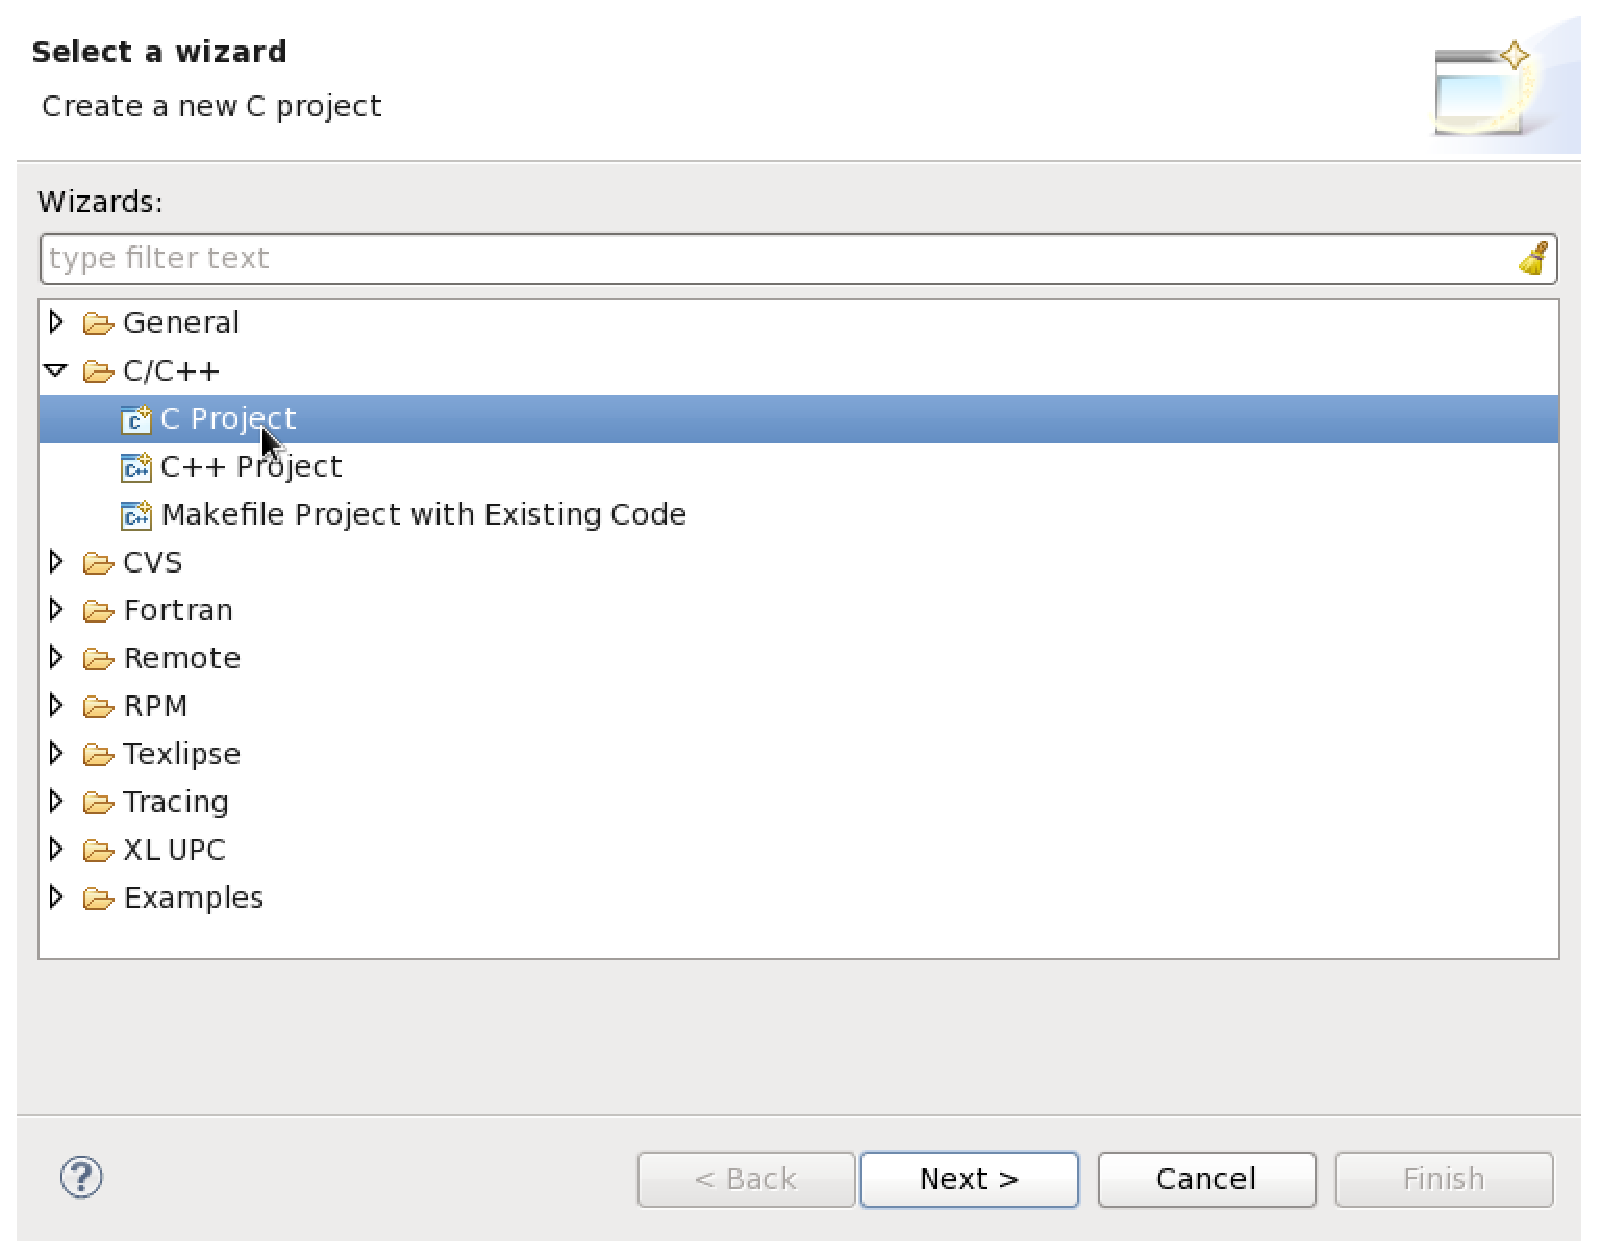
\includegraphics[width=67mm, keepaspectratio]{figures/eps/newC.eps}\hspace{1cm}
	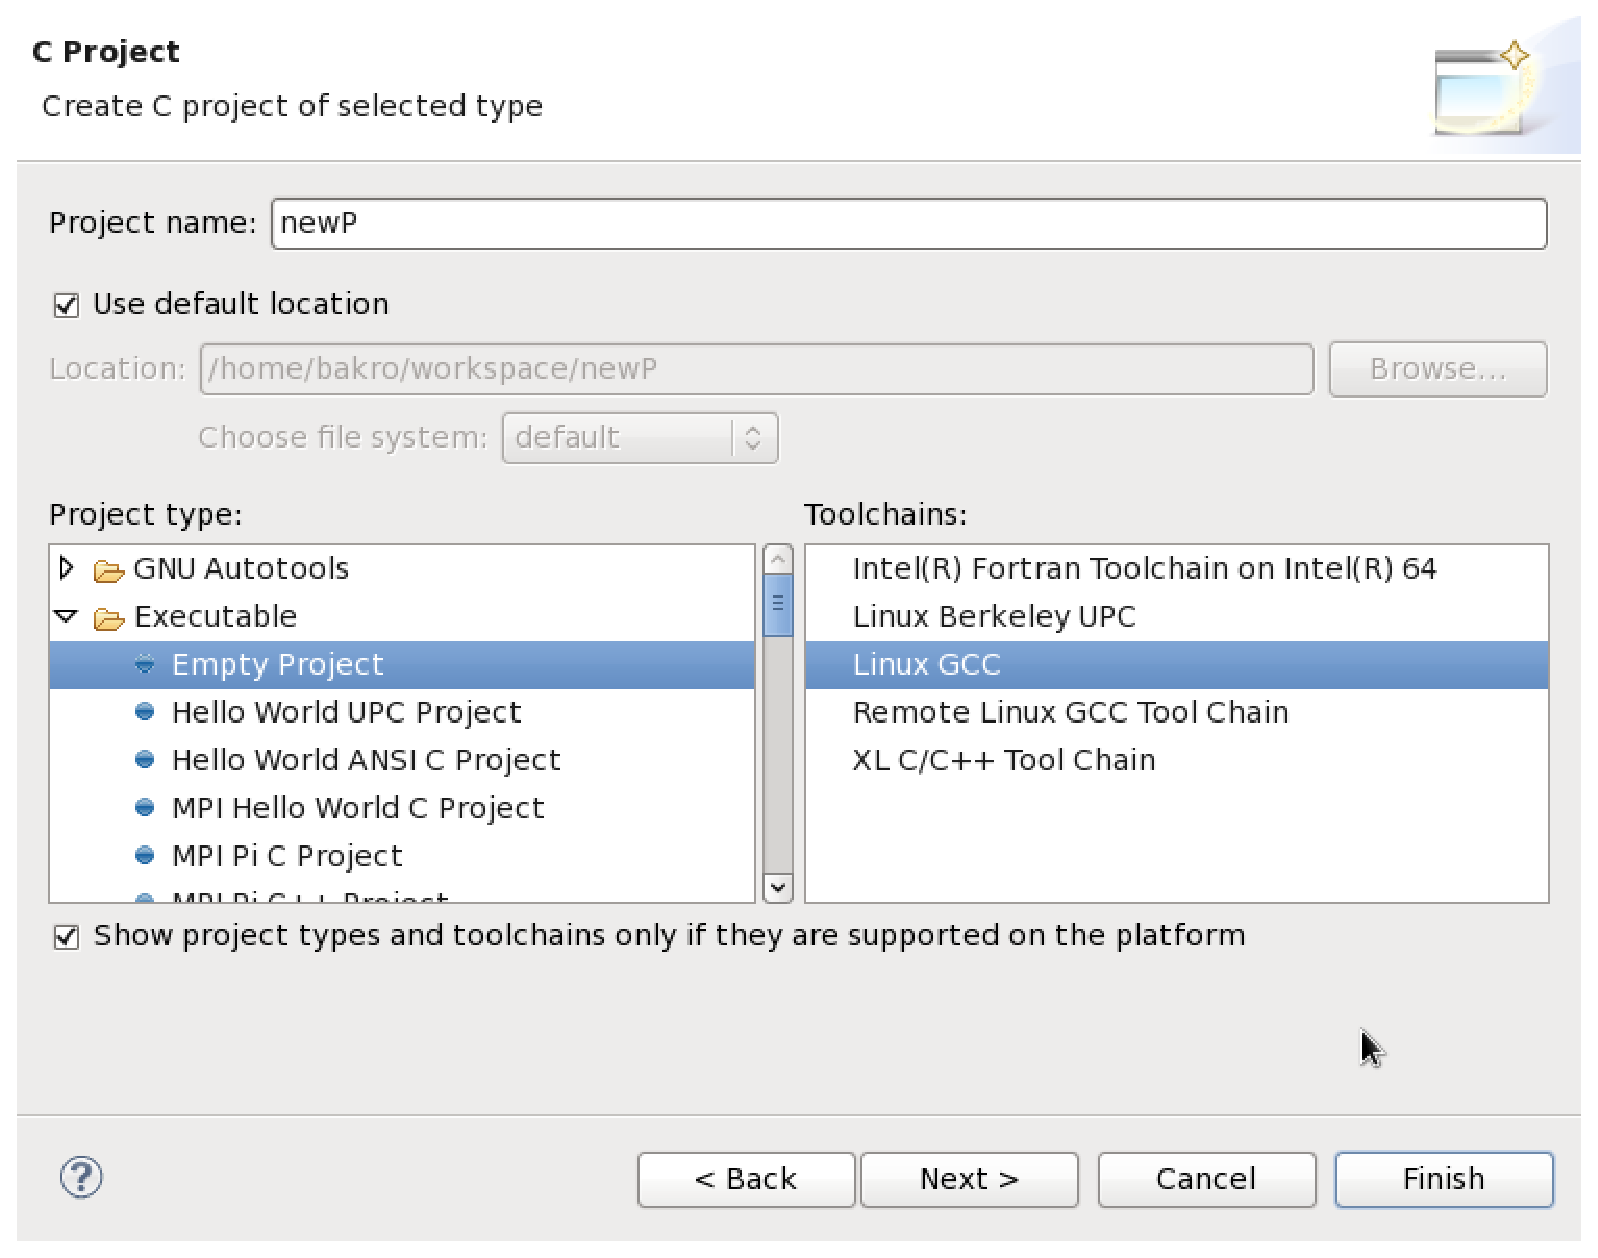
\includegraphics[width=67mm, keepaspectratio]{figures/eps/newP.eps}\\\vspace{5mm}
	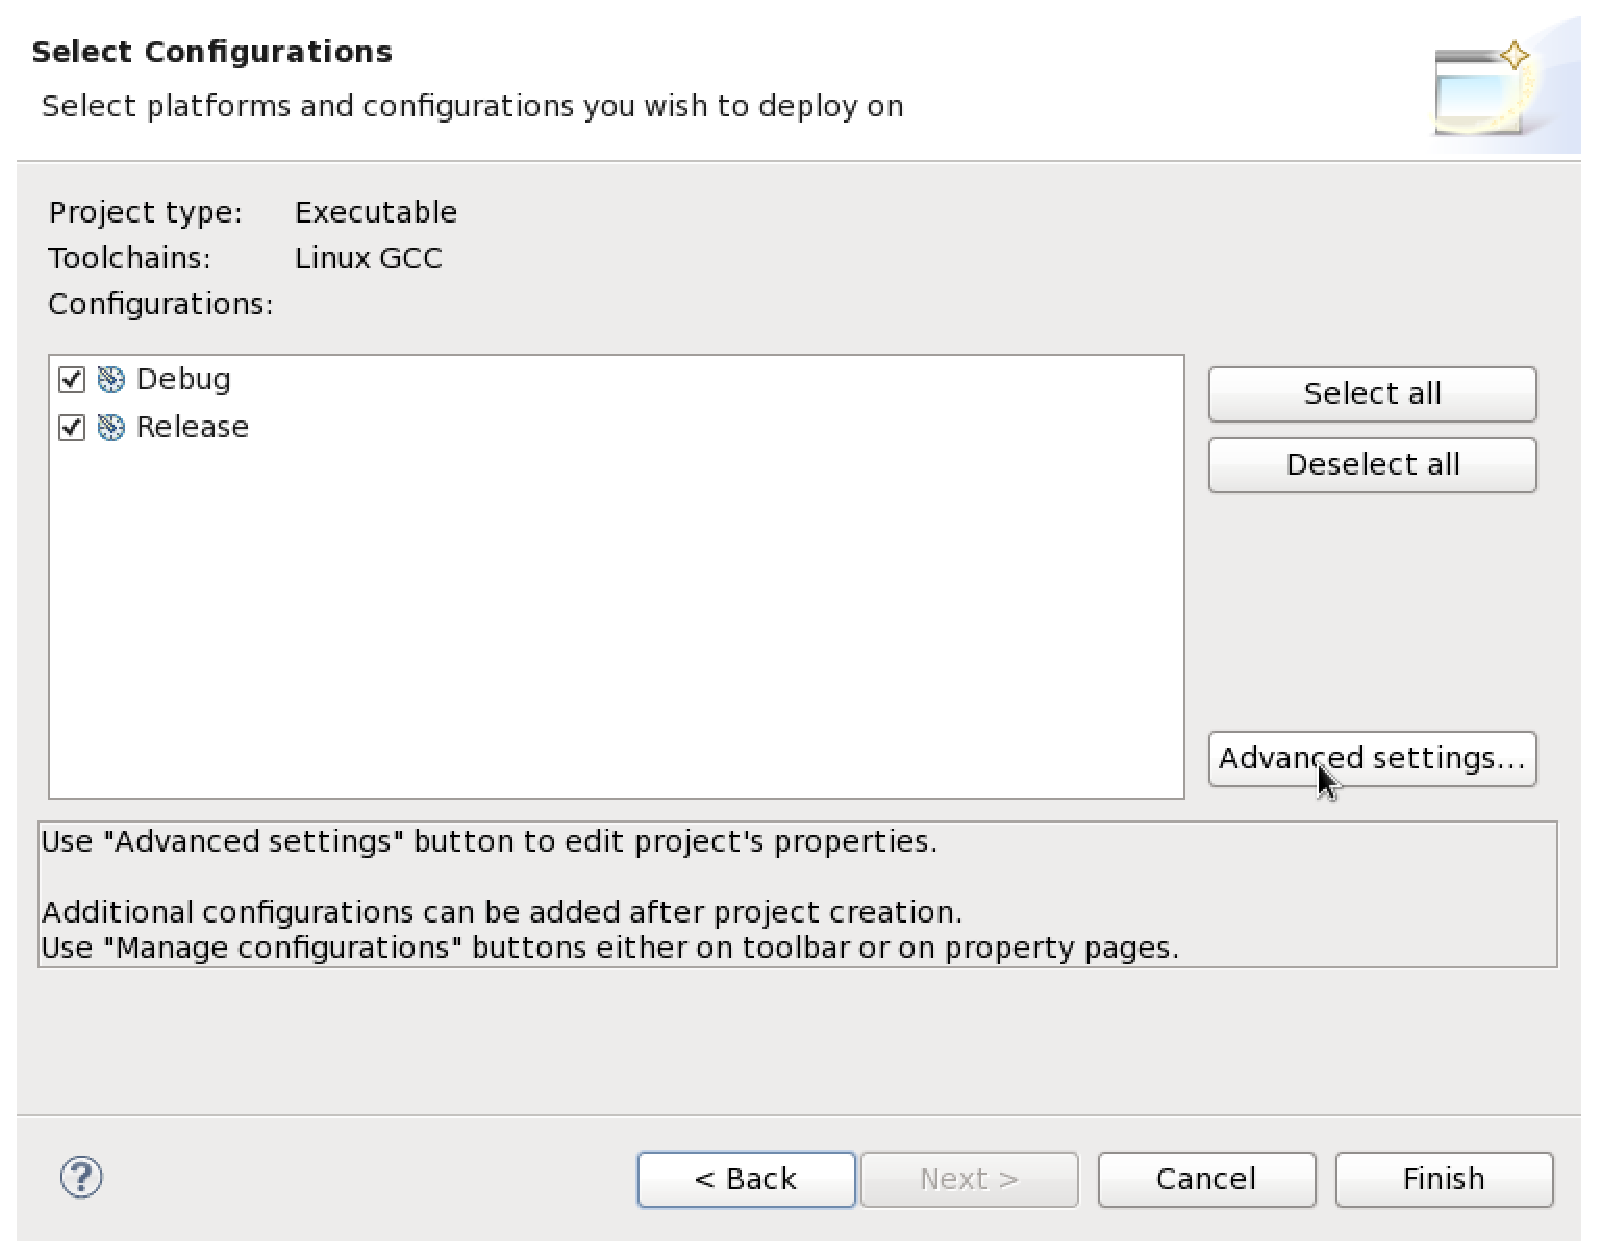
\includegraphics[width=67mm, keepaspectratio]{figures/eps/conf.eps}\hspace{1cm}
	\caption{Új Eclipse projekt létrehozása} 
	\label{fig:newproj}
	\end{figure}

\subsection{Compiler beállítása}
	A létrehozott projektre jobb gombbal kattíntva a tulajdonságára kattintva
	állíthatjuk be a fordítót a képnek \ref{fig:compiler} megfelelően.
	A beállítások kiterjednek a GNU-C99 nyelv szerinti fordításra és a korábbi
	\ref{sect:sdk} részben telepített SDK-ban található include mappa beállítására. 
	\begin{figure}[H]
	\centering
	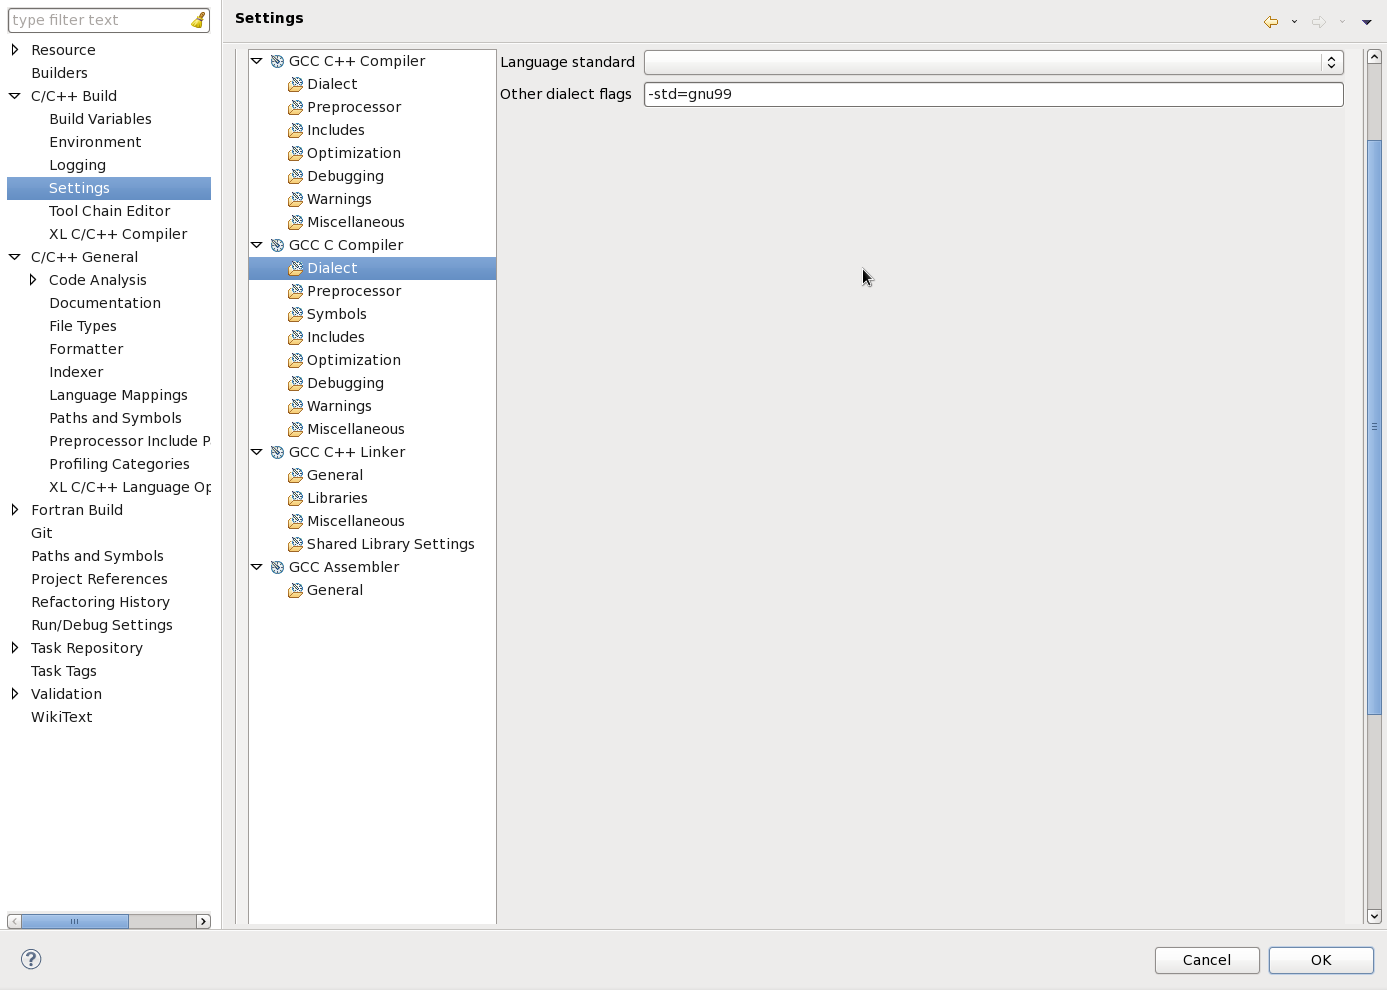
\includegraphics[width=67mm, keepaspectratio]{figures/eps/lang.eps}\hspace{1cm}
	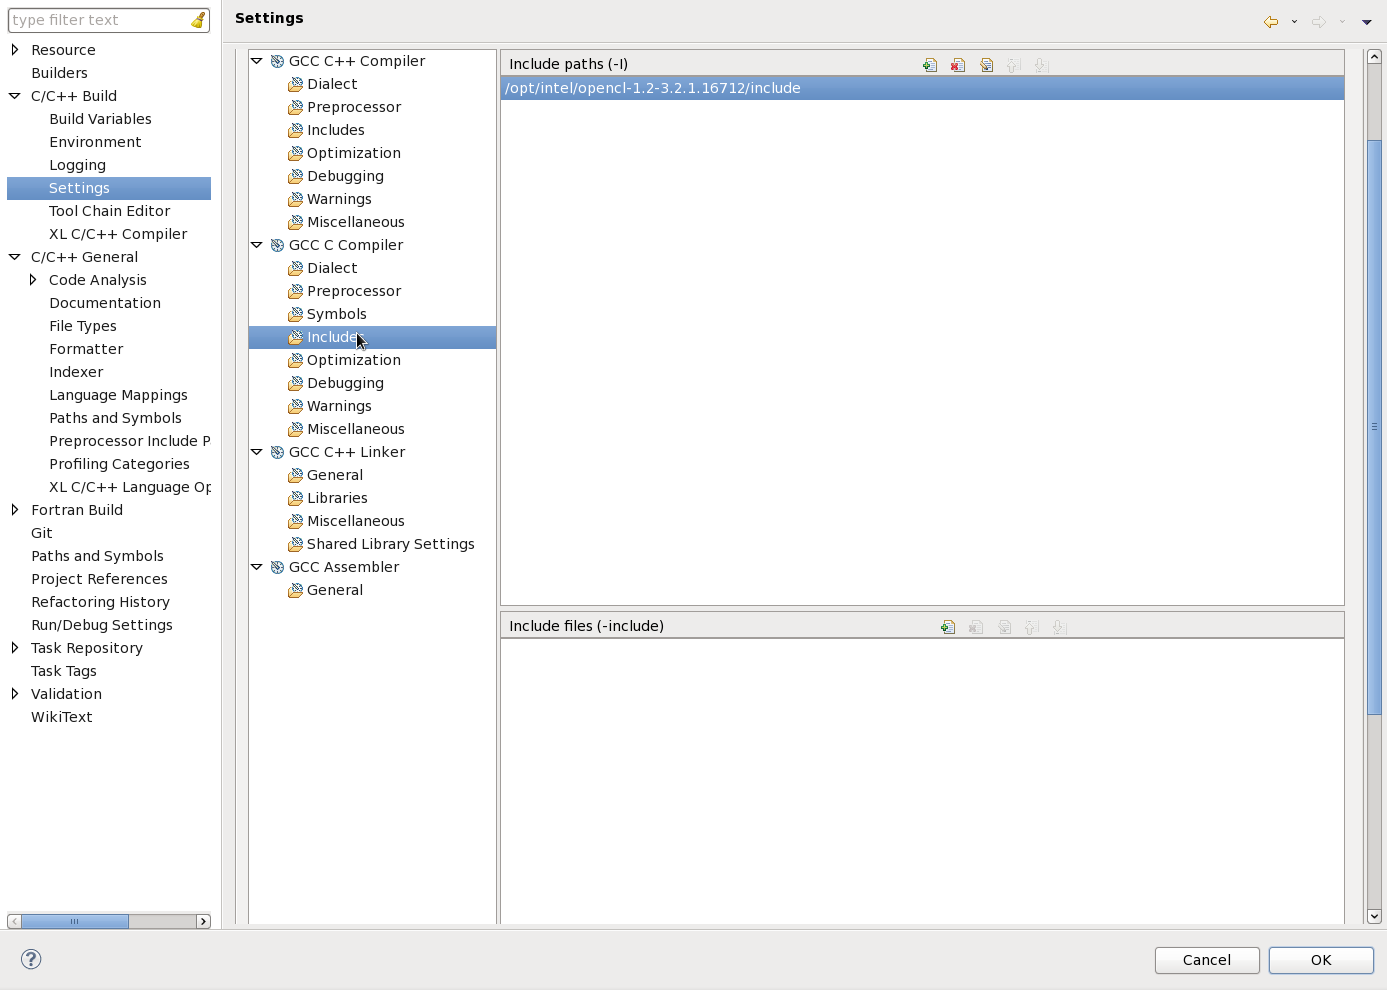
\includegraphics[width=67mm, keepaspectratio]{figures/eps/include.eps}\\\vspace{5mm}
	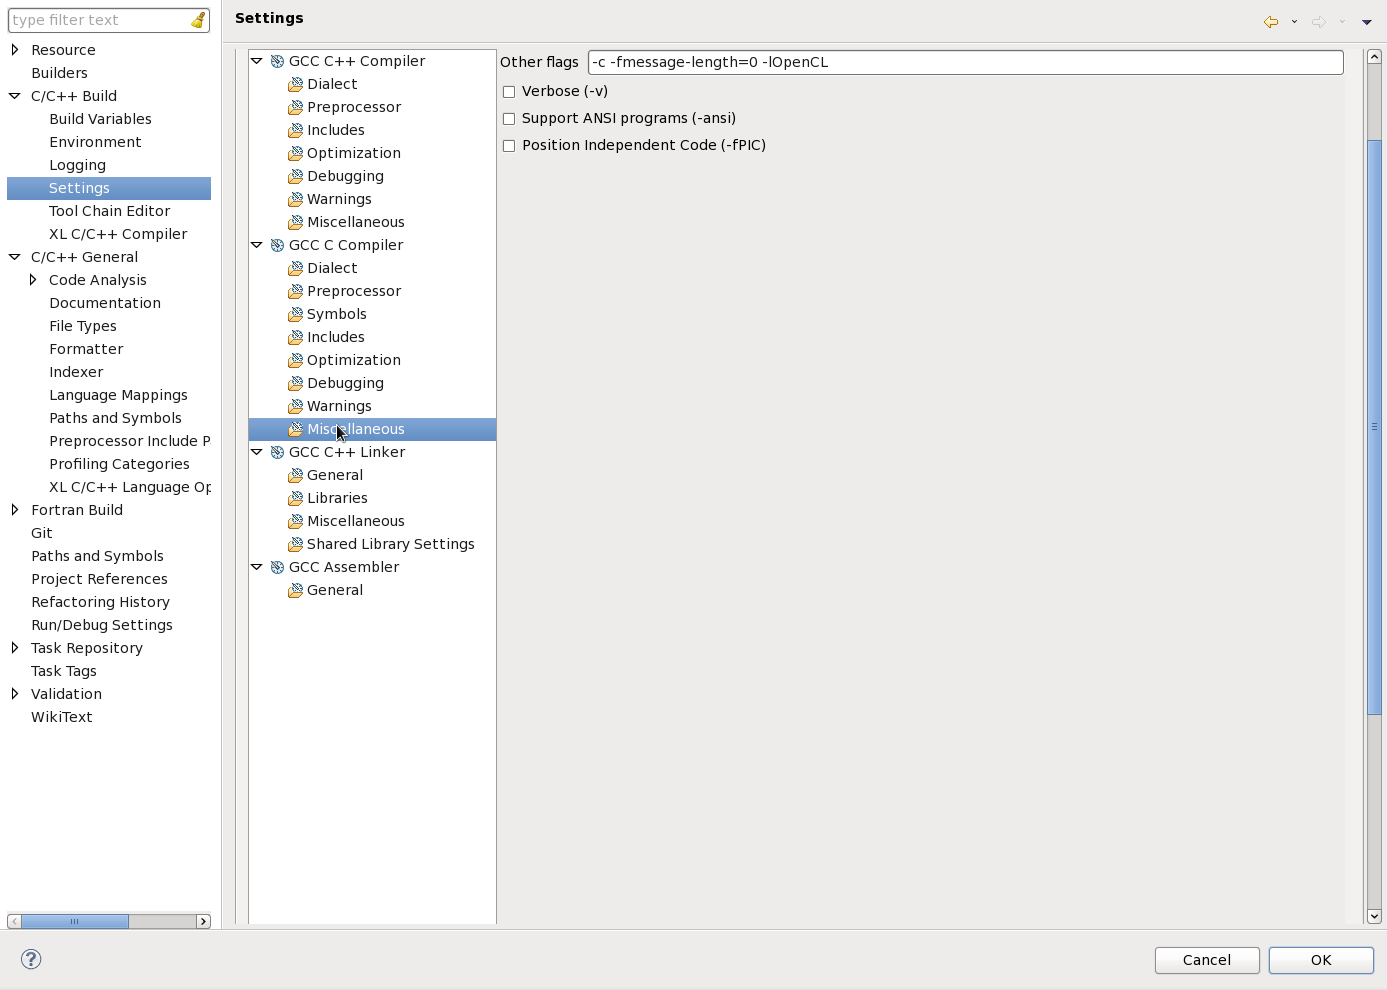
\includegraphics[width=67mm, keepaspectratio]{figures/eps/misc.eps}
	\caption{Compiler beállításai} 
	\label{fig:compiler}
	\end{figure}

\subsection{Linker beállítása}
	A linkert a \ref{fig:linker} ábra szerint állítjuk be.
	\begin{figure}[H]
	\centering
	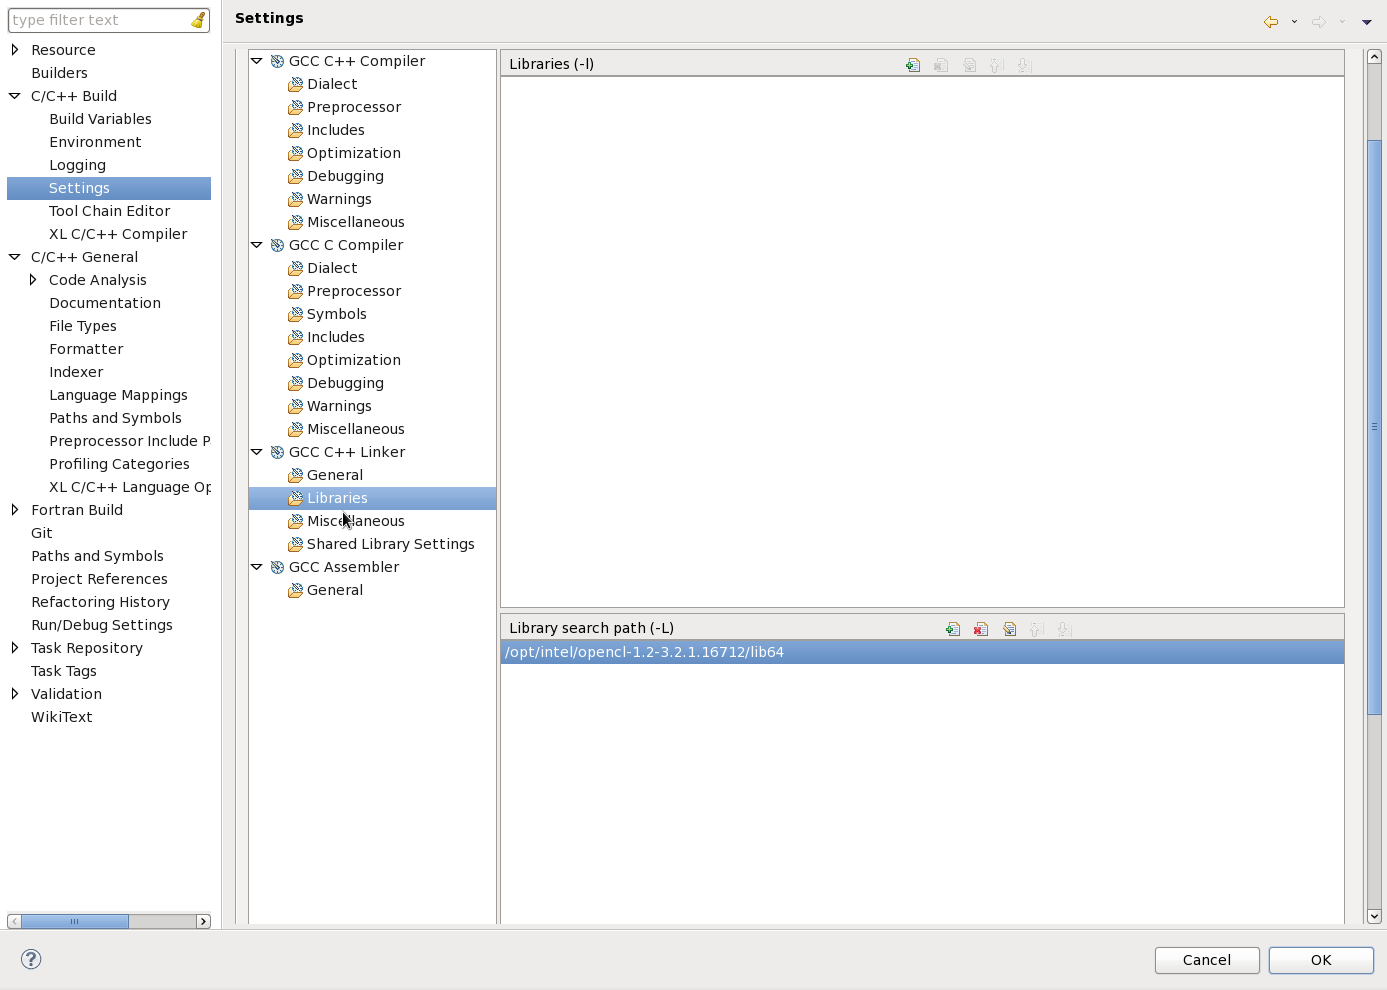
\includegraphics[width=67mm, keepaspectratio]{figures/eps/link.eps}\hspace{1cm}
	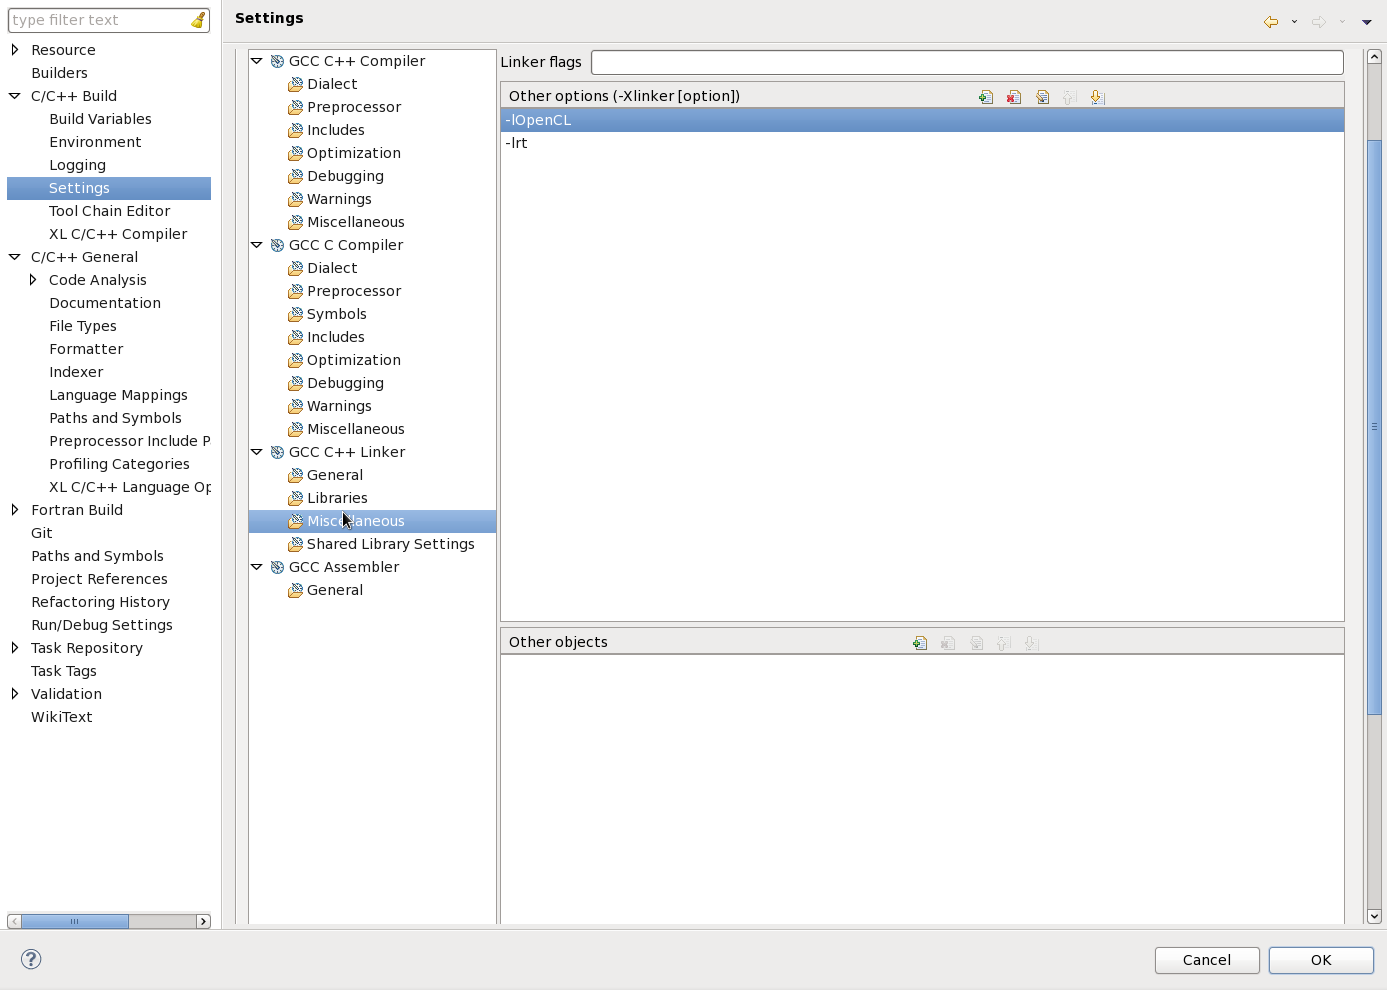
\includegraphics[width=67mm, keepaspectratio]{figures/eps/link_misc.eps}\\\vspace{5mm}
	\caption{Linker beállításai} 
	\label{fig:linker}
	\end{figure}


% ----------------------------------------------------------------------------
\chapter{Multiprocesszoros program}
% ----------------------------------------------------------------------------
\section{A program lépéseinek bemutatása}
	A $100\ \mathrm{FPS}$-el érkező képeket \textbf{tizesével} dolgozom fel, mivel a megjelenítésnek
	nem fontos real-time működésűnek lennie. 
	A program ciklikusan a következő lépéseket hajtja végre:
	\begin{enumerate*}
		\item Képek beolvasása a host-memóriába,
		\item Képek leküldése a host-memóriájábó az eszköz globális memóriájába,
		\item Eszközön futtatandó kernel inicializálása, argumentumainak beállítása,
		\item Kernel futtatása az eszközön,
		\item Kernel futása után az eredmény az eszköz globális memóriájából a host-memóriájába való
		visszatöltése,
		\item Posztprocesszálás,
	\end{enumerate*}
	A kernel megírása során a korábbi \ref{sec:opencl}. részben említetteket figyelembe kell venni.
	Főként a véges lokális és globális memóriát. A kernel adat-parallel módon lett megírva.
	A lokális memória $16 \mathrm{KByte}$ méretű, amit két $8 \mathrm{KByte}$ nagyságú $A$ és $B$
	bufferre osztottam fel.
	
	\noindent A kernel program lépései a következők:
	\begin{enumerate*}
		\item A work-item globális és lokális indexének meghatározása,
		\item Medián szűrés:
		\begin{enumerate*}
			\item A kép egy részének a globális memóriából a lokális $A$ bufferbe való másolása,
			\item Az összes work-item másolási folyamatának megvárása,
			\item Medián szűrés az $A$ bufferből a $B$ bufferba,
			\item Az $A$ bufferba az eredeti ($A$ buffer) és a szűrt ($B$ buffer) különbségének az eredményét
			(differenciális kép) elhelyezni,
			\item Döntési szint számítása és detektálás/megjelölés a $B$ bufferba,
			\item A $B$ bufferben lévő eredmény a globális memóriába való kiírása hibakeresés biztosítása
			végett.
		\end{enumerate*}
		\item Kiterjesztés és a flood-fill algoritmussal a ROI meghatározása:
		\begin{enumerate*}
			\item Megjelölt pixel keresése,
			\item Adott környezetére való kiterjesztése,
			\item A kiterjesztés során a két legtávolabbi pont lesz a ROI határpontjai.
		\end{enumerate*}
		\item Részecske pozíciójának számítása momentum módszerrel,
		\item Eredmény mentése a globális memóriába
	\end{enumerate*}
	
	A kernel lefutása után az eszköz globális memóriájából az eredményeket a hoszt-memóriájába töltjük.
	A számításigényes szűrés, detektálás és momentum számítás az eszközön hajtódott végre. A részecskék
	pozíciójának eloszlásának számítása memóriaigényes, de nem számításigényes feladat, így az a
	host-programban került megvalósításra.

	
% \begin{lstlisting}[frame=single,float=!ht,caption=A detektálás kernelének kódja,
% label=listing:kernel]
% asd;
% \end{lstlisting}
%----------------------------------------------------------------------------
\chapter{Összehasonlítás}
%----------------------------------------------------------------------------

	\begin{table}[!ht]
	\footnotesize
	\centering
	\caption[Eszközök futási idejének összehasonlítása]{Az eszközök erőforrásainak és a rajta futtatott
	programok futási idejének összehasonlítása.}
	\label{table:results}
	\setlength{\extrarowheight}{8pt}
% 		\begin{tabular}{ l | r | r | r | r}
% 		 & Intel Core i5 & nVidia GT330M & Intel Xeon & Xeon PHI \\ \hline
% 		MAX COMPUTE UNITS & $4$ & $6$ & $8$ & $224$\\
% 		MAX CLOCK FREQUENCY & 2400 & 1265 & 3000 & 1100\\
% 		MAX WORK GROUP\_SIZE & $8192$ & $512$ & $8192$ & $8192$ \\ \hline\hline
% 		GLOBAL MEM SIZE & $\sim 4Gbyte$ & $1Gbyte$ & $8Gbyte$ & $\sim 4.5Gbyte$\\
% 		LOCAL MEM SIZE & $32 Kbyte$ & $16 Kbyte$ & $32 Kbyte$ & $32 Kbyte$\\ \hline\hline
% 		Futási idő &
% 		\end{tabular}
	\begin{tabular}{ l | r | r}
		 & Intel Core i5 & nVidia GT330M \\ \hline
		MAX COMPUTE UNITS & $4$ & $6$\\
		MAX CLOCK FREQUENCY & 2400 & 1265 \\
		MAX WORK GROUP\_SIZE & $8192$ & $512$ \\ \hline\hline
		GLOBAL MEM SIZE & $\sim 4Gbyte$ & $1Gbyte$\\
		%MAX\_CONSTANT\_BUFFER\_SIZE & $131072$ & $65536$ & $131072$ & $131072$\\
		LOCAL MEM SIZE & $32 Kbyte$ & $16 Kbyte$\\ \hline\hline
		Futási idő & 1 & 2
	\end{tabular}
	\end{table}




%\include{chapter6}
%\include{chapter7}
%----------------------------------------------------------------------------
\chapter{Összegzés}
%----------------------------------------------------------------------------

	Dolgozatomban bemutattam a porosplazma kísérletek apparátusát. A kísérlet során a kristályrácsba
	rendeződő részecskékről egy nagysebességű kamerával fényképek készülnek. A dolgozatomban ezen
	képeket, kellett feldolgoznom és a részecskék pozícióját detektálnom.
	A pozíciók a fizikai modell/szimuláció validálására szolgálnak.
	
	Ismertettem a részecske detektálásának módszerét szűrés és adaptív döntési küszöb használatával.
	Az elterjedt FIR Gauss szűrő helyett a hatékonyabb medián szűrőt javasoltam és alkalmaztam. A
	pozíció számítására a momentum módszert implementáltam, ami nagyobb számítási energiát igényel, de
	szubpixeles felbontást tudtam vele elérni. Konstatáltam, hogy az így kialakult program masszívan párhuzamosítható.
	
	Ezután áttekintettem az OpenCL keretrendszert, amit a párhuzamos program megírásának segítségére
	használtam. Az itt ismertetett megállapításokat figyelembe véve állítottam össze a párhuzamos
	program lépéseit, amit részleteztem is.
	
	Végül az elkészült programot CPU-n és GPU-n is futtatva a futási idejüket összevetettem és
	azonosítottam a gyorsulás forrását kitérve a processzormagra és a memóriájára.
	
	\section*{További feladatok:}
	\begin{itemize}
		\item A host-program real-time mérésbe helyezése egy producer-consumer sémájú szál megoldás
		alkalmazásával,
		\item Az eredmény grafikus  megjelenítése pl.: OpenGL használtatával,
		\item Az OpenCL szabvány által specifikált vektor műveletek támogatásának kiaknázása, ami az Intel
		Xeon PHI processzorkártyában rejlő teljesítményt ki tudná aknázni.
	\end{itemize}
	
	


\pagenumbering{Roman}
\setcounter{page}{1}
% \include{acknowledgement}
% 
\chapter{Függelék}


%----------------------------------------------------------------------------
\section{Matlab szimulátor}
%----------------------------------------------------------------------------
\texttt{feszko.m }
\begin{lstlisting}[frame=single]  % Start your code-block

clear all; close all; clc;

L = 1;

N = 500;
dx = L / N;

f0 = 0;
f1 = 1;

IT = 10000;

%%

fi = zeros(IT, N);
fi(:, 1) = f0 * ones(IT, 1);
fi(:, end) = f1 * ones(IT, 1);

T = zeros(N, N);
for n = 2:N-1
    T(n-1, n) =  0.5;
    T(n+1, n) =  0.5;
end
T(1,1) = 1;
T(end,end) = 1;

tic

for i = 2:IT
   fi(i, :) =  fi(i-1, :) * T;
end

toc

figure;
ax1 = subplot(211);
plot(linspace(0, L, N), fi(end, :)); grid;
xlabel('x');
ylabel('phi(x)');
title('Potencial eloszlas az iteracio vegen');

ax2 = subplot(212);
plot(linspace(0, L, N-1), diff(fi(end, :)) ./ dx);  grid;
xlabel('x');
ylabel('E(x)');
title('Elektromos ter az iteracio vegen');

linkaxes([ax1 ax2], 'x');

mfig(fi(1:1000:IT,1:4:N), 1:1000:IT,1:4:N)
\end{lstlisting}

\texttt{feszko2D.m }
\begin{lstlisting}[frame=single]  % Start your code-block

clear all; close all; clc;

X = 500;
Y = 500;

% mindig oszthato legyen 2vel
%global NX NY;
NX = 12;
NY = 12;

dx = X / NX;
dy = Y / NY;

f0 = 0;
f1 =1;


IT = 20000;

%%
ij2n = ((ones(NY,1) * (1:NX)) + ((0:NX:NX*(NY-1))' * ones(1,NX)))';


index = zeros(NX, NY);

index( 1: NX/4, NY/4+1:end) = -5;
index((3*NX/4)+1:end, 1: 3*NY/4) = -5;

index(1: 3*NX/4, 1) = -2;
index(3*NX/4, 1: 3*NY/4) = -6;
index(3*NX/4:end, (3*NY/4)+1) = -2;
index(end, (3*NY/4)+1 : end) = -6;
index((NX/4)+1:end, end) = -8;
index((NX/4)+1, NY/4:end) = -4;
index(1:NX/4, NY/4) = -8;
index(1, 1: NY/4) = -4;

index(3*NX/4,1) = -3;
index(3*NX/4,(3*NY/4)+1) = -3;

index((NX/4)+1,NY/4) = -7;
index((NX/4)+1,end) = -7;

index(1, 1:NY/4) = -10;
index(end, (3*NY/4)+1:end) = -11;


flip(index', 1)
flip(ij2n', 1)

%%
T = zeros(NX*NY, NX*NY);
[ii, jj] = find(index == 0);

for n = 1: length(ii)
    nn = ij2n(ii(n), jj(n));
    T(ij2n(ii(n)+1, jj(n)  ) , nn ) = 0.25;
    T(ij2n(ii(n)  , jj(n)+1) , nn ) = 0.25;
    T(ij2n(ii(n)-1, jj(n)  ) , nn ) = 0.25;
    T(ij2n(ii(n)  , jj(n)-1) , nn ) = 0.25;
end

valind = [ 1  1;
        0  1;
       -1  1;
        1  0;
        NaN NaN;
       -1  0;
        1 -1;
        0 -1;
       -1 -1];
        

% mi mivel
m = 1;
for i = 1:NX
    for j=1:NY
        if(-10 < index(i,j) & index(i,j) < 0 & index(i,j) ~= -5)
            mm(m, 1) = ij2n(i,j);
            mm(m, 2) = ij2n(i+valind(-index(i,j),1), j+valind(-index(i,j),2));
            m = m + 1;
        end
    end
end

f00 = find(reshape(index, 1, []) == -10);
f11 = find(reshape(index, 1, []) == -11);

%%
fi = zeros(IT, NX*NY);
% dirich
   for m= 1:length(f00)
       fi(1, f00(m)) = f0;
   end
   for m= 1:length(f11)
       fi(1, f11(m)) = f1;
   end

tic

for i = 2:IT
   fi(i, :) =  fi(i-1, :) * T;
   for m=1:length(mm)
       fi(i, mm(m, 1)) = fi(i, mm(m, 2));
   end
   % dirich
   for m= 1:length(f00)
       fi(i, f00(m)) = f0;
   end
   for m= 1:length(f11)
       fi(i, f11(m)) = f1;
   end
end

toc

fii = zeros(NX,NY, IT);
for i= 1:IT
    fii(:,:, i) = reshape(fi(i, :), NX, NY);
end



%%
fii( 1: NX/4, NY/4+1:end, end) = NaN;
fii((3*NX/4)+1:end, 1: 3*NY/4, end) = NaN;

figure;
ax1 = subplot(211);
contourf(fii(:,:,end)');
xlabel('x');
ylabel('y');
title('Potencial eloszlas az iteracio vegen');

ax2 = subplot(212);
contourf(diff(fii(:,:,end))');
xlabel('x');
ylabel('y');
title('Elektromos ter az iteracio vegen');

linkaxes([ax1 ax2], 'x');

%%


figm = figure('Renderer','zbuffer');
contourf(fii(:,:,2)'); title('0');
axis tight
set(gca,'NextPlot','replaceChildren');
% Preallocate the struct array for the struct returned by getframe
F(200) = struct('cdata',[],'colormap',[]);
% Record the movie
for j = 1:200
    fii( 1: NX/4, NY/4+1:end, j*100) = NaN;
    fii((3*NX/4)+1:end, 1: 3*NY/4, j*100) = NaN;
    surf(fii(:,:,j*100)');
    title(['it = ' num2str(j*100)]);
    xlabel('N'); ylabel('IT');
    
    %contourf(fii(:,:,j*100)'); 
    F(j) = getframe;
end


figure;
movie(F, 2)
\end{lstlisting}


\texttt{main.cu}
\begin{lstlisting}[frame=single]  % Start your code-block

#include <stdio.h>
#include <stdlib.h>
#include <time.h>
#include <string.h>

#include <helper_functions.h>
#include <helper_cuda.h>


extern "C"
void CPU(
    float *h_C,
    float *h_A,
    float *h_B,
    int vectorN,
    int elementN
);



#include "kernel.cuh"


float RandFloat(float low, float high)
{
    float t = (float)rand() / (float)RAND_MAX;
    return (1.0f - t) * low + t * high;
}



///////////////////////////////////////////////////////////////////////////////
// Data configuration
///////////////////////////////////////////////////////////////////////////////

const int VECTOR_N = 456;
const int ELEMENT_N = 4096;

const int    DATA_N = VECTOR_N * ELEMENT_N;

const int   DATA_SZ = DATA_N * sizeof(float);
const int RESULT_SZ = VECTOR_N  * sizeof(float);



///////////////////////////////////////////////////////////////////////////////
// Main program
///////////////////////////////////////////////////////////////////////////////
int main(int argc, char **argv)
{
    float *h_A, *h_B, *h_C_CPU, *h_C_GPU;
    float *d_A, *d_B, *d_C;
    //double delta, ref, sum_delta, sum_ref, L1norm;
    StopWatchInterface *hTimer = NULL;
    int i;


	getchar();

    printf("%s Starting...\n\n", argv[0]);

    // use command-line specified CUDA device, otherwise use device with highest Gflops/s
    findCudaDevice(argc, (const char **)argv);

    sdkCreateTimer(&hTimer);

    printf("Initializing data...\n");
    printf("...allocating CPU memory.\n");
    h_A     = (float *)malloc(DATA_SZ);
    h_B     = (float *)malloc(DATA_SZ);
    h_C_CPU = (float *)malloc(RESULT_SZ);
    h_C_GPU = (float *)malloc(RESULT_SZ);

    printf("...allocating GPU memory.\n");
    checkCudaErrors(cudaMalloc((void **)&d_A, DATA_SZ));
    checkCudaErrors(cudaMalloc((void **)&d_B, DATA_SZ));
    checkCudaErrors(cudaMalloc((void **)&d_C, RESULT_SZ));

    printf("...generating input data in CPU mem.\n");
    srand(123);

    //Generating input data on CPU
    for (i = 0; i < DATA_N; i++)
    {
        h_A[i] = RandFloat(0.0f, 1.0f);
        h_B[i] = RandFloat(0.0f, 1.0f);
    }

    printf("...copying input data to GPU mem.\n");
    //Copy options data to GPU memory for further processing
    checkCudaErrors(cudaMemcpy(d_A, h_A, DATA_SZ, cudaMemcpyHostToDevice));
    checkCudaErrors(cudaMemcpy(d_B, h_B, DATA_SZ, cudaMemcpyHostToDevice));
    printf("Data init done.\n");


    printf("Executing GPU kernel...\n");
    checkCudaErrors(cudaDeviceSynchronize());
    sdkResetTimer(&hTimer);
    sdkStartTimer(&hTimer);
    GPU<<<128, 256>>>(d_C, d_A, d_B, VECTOR_N, ELEMENT_N);
    getLastCudaError("scalarProdGPU() execution failed\n");
    checkCudaErrors(cudaDeviceSynchronize());
    sdkStopTimer(&hTimer);
    printf("GPU time: %f msecs.\n", sdkGetTimerValue(&hTimer));

    printf("Reading back GPU result...\n");
    //Read back GPU results to compare them to CPU results
    checkCudaErrors(cudaMemcpy(h_C_GPU, d_C, RESULT_SZ, cudaMemcpyDeviceToHost));


    printf("Checking GPU results...\n");
    printf("..running CPU scalar product calculation\n");

	sdkResetTimer(&hTimer);
    sdkStartTimer(&hTimer);
    CPU(h_C_CPU, h_A, h_B, VECTOR_N, ELEMENT_N);
	 sdkStopTimer(&hTimer);
    printf("cPU time: %f msecs.\n", sdkGetTimerValue(&hTimer));


    
    exit(EXIT_SUCCESS);
}
\end{lstlisting}


\texttt{kernel.cuh}
\begin{lstlisting}[frame=single]  % Start your code-block

#define IMUL(a, b) __mul24(a, b)



#define ACCUM_N 1024
__global__ void GPU(
    float *d_C,
    float *d_A,
    float *d_B,
    int vectorN,
    int elementN
)
{
    //Accumulators cache
    __shared__ float accumResult[ACCUM_N];

    for (int vec = blockIdx.x; vec < vectorN; vec += gridDim.x)
    {
        int vectorBase = IMUL(elementN, vec);
        int vectorEnd  = vectorBase + elementN;

        for (int iAccum = threadIdx.x; iAccum < ACCUM_N; iAccum += blockDim.x)
        {
            float sum = 0;

            for (int pos = vectorBase + iAccum; pos < vectorEnd; pos += ACCUM_N)
                sum += d_A[pos] * d_B[pos];

            accumResult[iAccum] = sum;
        }

        for (int stride = ACCUM_N / 2; stride > 0; stride >>= 1)
        {
            __syncthreads();

            for (int iAccum = threadIdx.x; iAccum < stride; iAccum += blockDim.x)
                accumResult[iAccum] += accumResult[stride + iAccum];
        }

        if (threadIdx.x == 0) d_C[vec] = accumResult[0];
    }
}
\end{lstlisting}

 

\listoffigures\addcontentsline{toc}{chapter}{Ábrák jegyzéke}
\listoftables\addcontentsline{toc}{chapter}{Táblázatok jegyzéke}

\bibliography{diploma1.bib}
\addcontentsline{toc}{chapter}{Irodalomjegyzék}
\bibliographystyle{ieeetr}



\label{page:last}
\end{document}
